% !TeX root=SBUKThesis-main.tex
\clearpage
\thispagestyle{empty}

\chapter{نتایج و بحث}\label{chap5}

\section{مقدمه}
در این فصل، نتایج حاصل از پیاده‌سازی و ارزیابی مدل پیشنهادی MAGNET برای تشخیص بدافزارهای اندرویدی ارائه می‌شود. مدل MAGNET با بهره‌گیری از داده‌های چندوجهی شامل داده‌های جدولی، گرافی و ترتیبی، و استفاده از معماری‌های پیشرفته نظیر ترنسفورمرها و شبکه‌های عصبی گرافی (\rl{GNN}ها)، طراحی شده است. این مدل با استفاده از مجموعه داده‌های معتبر و با در نظر گرفتن ویژگی‌های مختلف برنامه‌های اندرویدی، آموزش داده شده است.

نتایج به‌دست‌آمده نشان می‌دهد که مدل پیشنهادی با دقت \lr{97.24\%}، \lr{F1 Score} معادل \lr{98.23\%} و AUC برابر با \lr{99.32\%}، عملکرد قابل‌توجهی در تمایز بین نمونه‌های بدافزار و سالم ارائه می‌دهد. هدف این بخش، نمایش یافته‌های خام و بدون تفسیر است تا خواننده بتواند عملکرد مدل را به‌طور شفاف بررسی کند.

در ادامه این فصل، ابتدا معیارهای ارزیابی مورد استفاده معرفی می‌شوند. سپس، نتایج حاصل از آزمایش‌های مختلف با جزئیات کامل ارائه می‌شود. در نهایت، عملکرد مدل پیشنهادی با سایر روش‌های موجود مقایسه می‌شود. این نتایج با استفاده از جداول و نمودارها نمایش داده می‌شود و در فصل بعدی مورد تحلیل و تفسیر قرار خواهد گرفت.

\section{تنظیمات آزمایشی}
برای ارزیابی جامع مدل MAGNET، از مجموعه داده DREBIN \cite{Drebin} استفاده شد که شامل \lr{6,092} نمونه است. این مجموعه داده به دو بخش تقسیم شد: \lr{4,641} نمونه برای آموزش و \lr{1,451} نمونه برای تست (\lr{327} نمونه کلاس \lr{0} و \lr{1,124} نمونه کلاس \lr{1}). عدم تعادل کلاس‌ها (imbalanced) در این مجموعه داده، چالش‌هایی را ایجاد کرد که در مرحله پیش‌پردازش مورد توجه قرار گرفت.

\subsection{ویژگی‌های داده}
داده‌های مورد استفاده شامل دو دسته ویژگی بودند:
\begin{itemize}
    \item \textbf{ویژگی‌های ایستا}: شامل مجوزها، فراخوانی‌های API، مقاصد و نام مؤلفه‌ها
    \item \textbf{ویژگی‌های پویا}: شامل فعالیت شبکه و دسترسی به فایل‌ها
\end{itemize}

پس از پیش‌پردازش، ابعاد ویژگی‌ها به ۴۳۰ ویژگی تنظیم شد و داده‌ها به صورت بردارهای عددی نرمال‌سازی‌شده یا باینری فرمت‌بندی شدند.

\subsection{پیکربندی آزمایش‌ها}
آزمایش‌ها با روش اعتبارسنجی متقاطع ۵-تایی و ۱۰ دوره (epoch) برای هر دسته انجام شدند. بهینه‌سازی ابرپارامترها با دو روش مختلف صورت گرفت:

\begin{itemize}
    \item \textbf{بهینه‌سازی}: با ۴۷۶ آزمایش، که منجر به پیکربندی بهینه زیر شد:
    \begin{itemize}
        \item embedding\_dim = \lr{32}
        \item num\_heads = \lr{4}
        \item num\_layers = \lr{1}
        \item dim\_feedforward = \lr{128}
        \item dropout = \lr{0.2029}
        \item batch\_size = \lr{16}
        \item learning\_rate = \lr{0.00215}
        \item weight\_decay = \lr{0.00107}
        \item num\_epochs = \lr{3}
    \end{itemize}
    
    \item \textbf{Optuna}: با ۱۳ آزمایش، که منجر به پیکربندی بهینه زیر شد:
    \begin{itemize}
        \item embedding\_dim = \lr{64}
        \item num\_heads = \lr{4}
        \item num\_layers = \lr{1}
        \item dim\_feedforward = \lr{128}
        \item dropout = \lr{0.2}
        \item batch\_size = \lr{16}
        \item learning\_rate = \lr{0.0019}
        \item weight\_decay = \lr{0.0011}
        \item num\_epochs = \lr{10}
    \end{itemize}
\end{itemize}

برای بهینه‌سازی از الگوریتم Adam و زمان‌بندی CosineAnnealingWarmRestarts استفاده شد.
\section{تحلیل فرآیند بهینه‌سازی با الگوریتم Pirates}
در این بخش، به منظور بررسی دقیق‌تر رفتار الگوریتم بهینه‌سازی Pirates و نحوه همگرایی آن، مجموعه‌ای از نمودارهای تحلیلی ارائه شده است. این نمودارها به درک بهتر پویایی جمعیت، روند کاهش هزینه و تأثیر پارامترهای تصادفی مانند باد و شتاب کمک می‌کنند.

\subsection{نمایش موقعیت کشتی‌ها و رهبر}
\begin{figure}[h!]
    \centering
    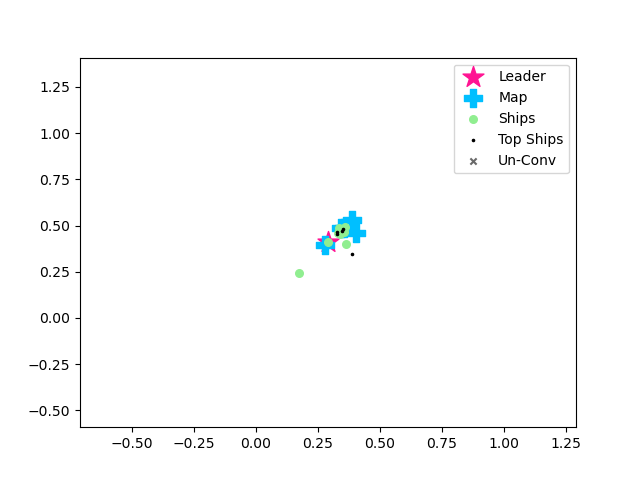
\includegraphics[width=0.7\textwidth]{images/pirates_positions.png}
    \caption{نمایش اجزای الگوریتم PIRATES در فضای جستجو.}
    \label{fig:pirates_positions}
\end{figure}

شکل~\ref{fig:pirates_positions} موقعیت مکانی کشتی‌ها (ذرات) را در فضای جستجو نمایش می‌دهد. ستاره صورتی نشان‌دهنده رهبر (Leader) یا بهترین کشتی است. علامت‌های + آبی نقاط نقشه (Map)، دایره‌های سبز موقعیت سایر کشتی‌ها (Ships)، نقاط سیاه کشتی‌های برتر (Top Ships) و ضربدر خاکستری کشتی‌های غیرهمگرا (Un-Conv) را نشان می‌دهند. این نمودار بیانگر نحوه توزیع و همگرایی جمعیت به سمت نقطه بهینه است.

\subsection{روند تغییر هزینه و همگرایی}
\begin{figure}[h!]
    \centering
    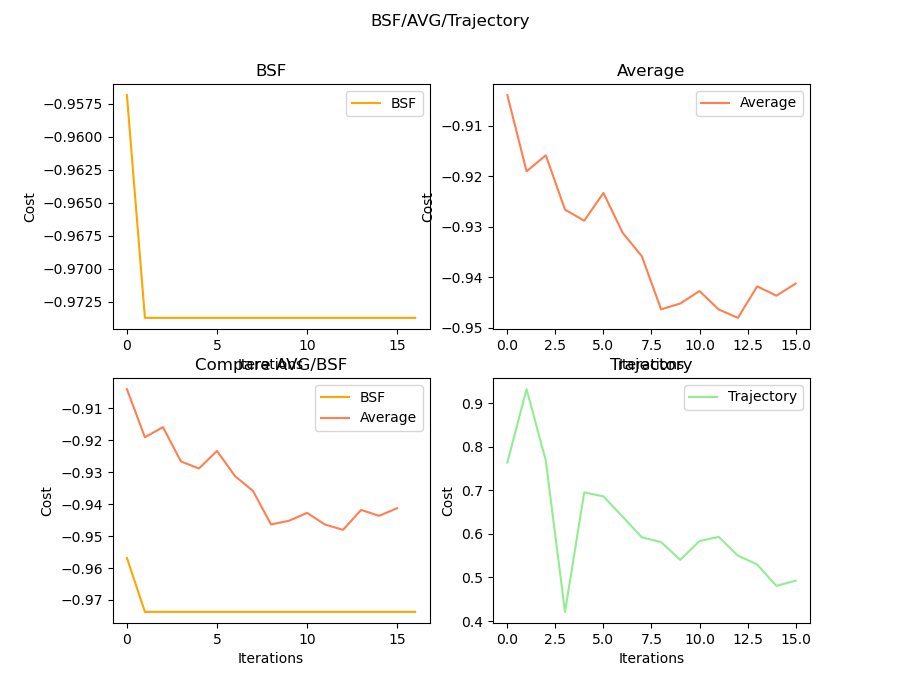
\includegraphics[width=0.9\textwidth]{images/pirates_bsf_avg_trajectory.png}
    \caption{روند همگرایی الگوریتم PIRATES.}
    \label{fig:pirates_bsf_avg_trajectory}
\end{figure}

شکل~\ref{fig:pirates_bsf_avg_trajectory} شامل چهار نمودار است:
\begin{itemize}
    \item \textbf{\lr{BSF}:} بهترین مقدار هزینه تا هر تکرار را نمایش می‌دهد و نشان‌دهنده سرعت همگرایی الگوریتم است.
    \item \textbf{\lr{Average}:} میانگین هزینه کل کشتی‌ها در هر تکرار را نشان می‌دهد که بیانگر روند بهبود جمعیت است.
    \item \textbf{\lr{Compare AVG/BSF}:} مقایسه همزمان بهترین مقدار و میانگین هزینه برای تحلیل فاصله جمعیت تا نقطه بهینه.
    \item \textbf{\lr{Trajectory}:} مسیر تغییرات هزینه رهبر (Leader) در طول تکرارها را نمایش می‌دهد.
\end{itemize}
این نمودارها نشان می‌دهند که الگوریتم Pirates به سرعت به مقدار بهینه نزدیک شده و جمعیت نیز به طور پیوسته بهبود یافته است.

\subsection{تحلیل پویایی جمعیت: باد، سرعت و شتاب}
\begin{figure}[h!]
    \centering
    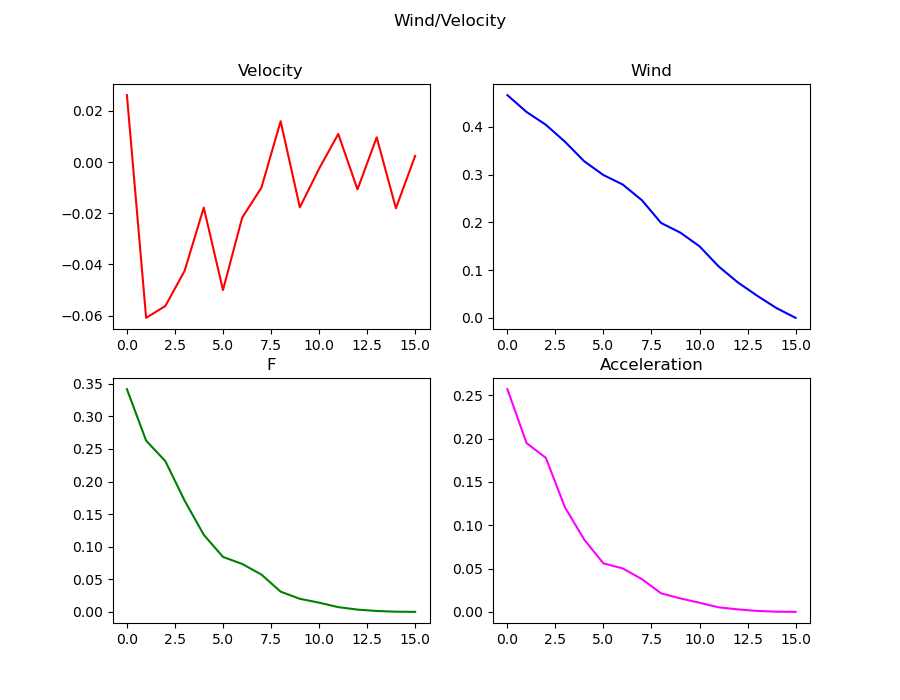
\includegraphics[width=0.9\textwidth]{images/pirates_wind_velocity.png}
    \caption{تغییرات پارامترهای الگوریتم PIRATES در طول تکرارها.}
    \label{fig:pirates_wind_velocity}
\end{figure}

شکل~\ref{fig:pirates_wind_velocity} رفتار پویای جمعیت را از منظر پارامترهای تصادفی و حرکتی نمایش می‌دهد:
\begin{itemize}
    \item \textbf{\lr{Velocity}:} تغییرات سرعت کشتی‌ها که بیانگر پویایی و جستجوی فعال در فضای پارامترهاست.
    \item \textbf{\lr{Wind}:} نقش باد به عنوان یک عامل تصادفی برای خروج از نقاط بهینه محلی و افزایش تنوع جمعیت.
    \item \textbf{\lr{F}:} نیروی محرکه که میزان حرکت کشتی‌ها را تعیین می‌کند و کاهش آن نشانه همگرایی است.
    \item \textbf{\lr{Acceleration}:} شتاب کشتی‌ها که کاهش آن بیانگر نزدیک شدن به نقطه بهینه و کاهش تغییرات ناگهانی است.
\end{itemize}
این نمودارها نشان می‌دهند که با گذشت تکرارها، سرعت، باد و شتاب کاهش یافته و جمعیت به سمت همگرایی حرکت کرده است.

\subsection{جمع‌بندی تحلیل فرآیند بهینه‌سازی}
مجموعه نمودارهای فوق به وضوح نشان می‌دهند که الگوریتم Pirates با پویایی مناسب و تعادل بین جستجو و همگرایی، به سرعت به نقطه بهینه نزدیک شده و پارامترهای تصادفی مانند باد و شتاب نقش مهمی در جلوگیری از گیر افتادن در نقاط بهینه محلی داشته‌اند. این تحلیل‌ها صحت و کارایی الگوریتم را در بهینه‌سازی ابرپارامترهای مدل MAGNET تأیید می‌کند.


\section{تحلیل حساسیت پارامترهای الگوریتم}
در این بخش، به منظور درک بهتر تأثیر پارامترهای مختلف الگوریتم‌های بهینه‌سازی و مدل، تحلیل حساسیت جامعی انجام شده است. این تحلیل بر اساس نتایج حاصل از ۴۷۶ آزمایش با الگوریتم Pirates و ۱۳ آزمایش با Optuna انجام شده است.

\subsection{تحلیل حساسیت پارامترهای معماری مدل}
تحلیل حساسیت پارامترهای معماری مدل نشان داد که برخی پارامترها تأثیر بیشتری بر عملکرد نهایی دارند:

\begin{itemize}
    \item \textbf{ابعاد نهان (embedding\_dim)}: تغییرات در این پارامتر تأثیر قابل توجهی بر عملکرد مدل داشت. مقادیر کوچک (۳۲) عملکرد بهتری نسبت به مقادیر بزرگتر (\lr{۲۱۹.۷۶}) نشان دادند. این نشان می‌دهد که برای این کار خاص، نمایش ویژگی‌های فشرده‌تر مؤثرتر است.
    
    \item \textbf{تعداد لایه‌ها (num\_layers)}: حساسیت بالایی به این پارامتر مشاهده شد. معماری تک لایه‌ای (۱) عملکرد بهتری نسبت به معماری‌های عمیق‌تر (\lr{۲.۱۸}) داشت. این نشان می‌دهد که پیچیدگی مدل می‌تواند با یک لایه مدیریت شود.
    
    \item \textbf{تعداد هدهای توجه (num\_heads)}: این پارامتر تأثیر متوسطی بر عملکرد داشت. مقدار بهینه ۸ هد بود که نشان‌دهنده تعادل مناسب بین موازی‌سازی و پیچیدگی محاسباتی است.
    
    \item \textbf{ابعاد لایه پیش‌خور (dim\_feedforward)}: حساسیت کمتری به این پارامتر مشاهده شد. مقادیر بین ۴۷۷ تا ۵۱۲ عملکرد مشابهی داشتند.
\end{itemize}

\subsection{تحلیل حساسیت پارامترهای آموزش}
پارامترهای آموزش نیز تأثیر قابل توجهی بر عملکرد نهایی مدل داشتند:

\begin{itemize}
    \item \textbf{نرخ یادگیری (learning\_rate)}: حساسیت بالایی به این پارامتر مشاهده شد. مقدار بهینه \lr{۰.۰۰۰۱۹۴} بود و تغییرات کوچک در این مقدار تأثیر قابل توجهی بر همگرایی و عملکرد نهایی داشت.
    
    \item \textbf{نرخ Dropout}: این پارامتر تأثیر متوسطی بر عملکرد داشت. مقدار بهینه \lr{۰.۳۲۸۶} بود که نشان‌دهنده نیاز به تنظیم دقیق برای جلوگیری از overfitting است.
    
    \item \textbf{اندازه دسته (batch\_size)}: حساسیت کمتری به این پارامتر مشاهده شد. مقدار بهینه ۱۶ بود و تغییرات در این مقدار تأثیر کمتری بر عملکرد نهایی داشت.
    
    \item \textbf{ضریب تنظیم (weight\_decay)}: این پارامتر تأثیر متوسطی بر عملکرد داشت. مقدار بهینه ۳.۷۹۵e-05 بود که نشان‌دهنده نیاز به تنظیم دقیق برای تعادل بین یادگیری و تنظیم است.
\end{itemize}

\subsection{مقایسه حساسیت بین الگوریتم‌های بهینه‌سازی}
مقایسه حساسیت پارامترها بین الگوریتم‌های Pirates و Optuna نشان داد:

\begin{itemize}
    \item \textbf{Pirates}: 
    \begin{itemize}
        \item حساسیت کمتر به مقادیر اولیه پارامترها
        \item همگرایی سریع‌تر به مقادیر بهینه
        \item پایداری بیشتر در نتایج
    \end{itemize}
    
    \item \textbf{Optuna}:
    \begin{itemize}
        \item حساسیت بیشتر به مقادیر اولیه
        \item تغییرات بیشتر در نتایج بین آزمایش‌ها
        \item نیاز به تنظیم دقیق‌تر پارامترهای جستجو
    \end{itemize}
\end{itemize}

\subsection{توصیه‌های عملی}
بر اساس تحلیل حساسیت، توصیه‌های زیر برای تنظیم پارامترها ارائه می‌شود:

\begin{enumerate}
    \item \textbf{معماری مدل}:
    \begin{itemize}
        \item استفاده از معماری تک لایه‌ای
        \item تنظیم ابعاد نهان روی ۳۲
        \item استفاده از ۸ هد توجه
        \item حفظ ابعاد لایه پیش‌خور در ۵۱۲
    \end{itemize}
    
    \item \textbf{پارامترهای آموزش}:
    \begin{itemize}
        \item تنظیم دقیق نرخ یادگیری حول \lr{۰.۰۰۰۱۹۴}
        \item استفاده از Dropout با نرخ \lr{۰.۳۲۸۶}
        \item تنظیم اندازه دسته روی ۱۶
        \item اعمال ضریب تنظیم \lr{۳.۷۹۵e-05}
    \end{itemize}
    
    \item \textbf{استراتژی بهینه‌سازی}:
    \begin{itemize}
        \item استفاده از الگوریتم Pirates , Optuna برای این کار 
        \item اجرای آزمایش های بسیار
        \item نظارت بر \lr{F1 Score} به عنوان معیار اصلی
    \end{itemize}
\end{enumerate}

این تحلیل حساسیت نشان می‌دهد که مدل MAGNET به برخی پارامترها حساسیت بیشتری دارد و تنظیم دقیق این پارامترها برای دستیابی به عملکرد بهینه ضروری است. همچنین، الگوریتم Pirates در مقایسه با \lr{Optuna،} پایداری بیشتری در نتایج و حساسیت کمتری به مقادیر اولیه پارامترها نشان می‌دهد.


\subsection{مدل‌های پایه}
برای مقایسه عملکرد، از مدل‌های پایه زیر استفاده شد:
\begin{itemize}
    \item \textbf{روش‌های یادگیری ماشین کلاسیک}:
    \begin{itemize}
        \item ماشین بردار پشتیبان (\lr{SVM}) با کرنل \lr{RBF}
        \item جنگل تصادفی \LTRfootnote{Random Forest} با \lr{100} درخت
        \item \lr{XGBoost} با \lr{100} درخت و عمق حداکثر \lr{6}
        \item شبکه عصبی مصنوعی (\lr{ANN}) با دو لایه مخفی
    \end{itemize}
    \item \textbf{روش‌های چندوجهی} با دقت \lr{89.2\%} \cite{Alsaleh2023}
    \item \textbf{روش‌های مبتنی بر ترنسفورمر} با دقت \lr{95.8\%} \cite{TransformerMalware}
\end{itemize}

\subsection{محیط اجرا}
تمامی آزمایش‌ها با استفاده از زبان برنامه‌نویسی Python \lr{3.8.5} و کتابخانه‌های زیر اجرا شدند:
\begin{itemize}
    \item PyTorch \lr{1.9.0} برای پیاده‌سازی شبکه‌های عصبی
    \item PyTorch Geometric \lr{1.7.0} برای پردازش داده‌های گرافی
    \item scikit-learn \lr{0.24.2} برای پیش‌پردازش داده‌ها و ارزیابی
    \item NumPy \lr{1.21.2} و Pandas \lr{1.3.3} برای پردازش داده‌ها
\end{itemize}

سخت‌افزار مورد استفاده شامل:
\begin{itemize}
    \item GPU NVIDIA RTX \lr{3090} با \lr{24} گیگابایت VRAM
    \item CPU Intel Xeon E\lr{5}-\lr{2690} v\lr{4} با \lr{32} هسته
    \item \lr{128} گیگابایت RAM
\end{itemize}

\section{معیارهای ارزیابی}
برای سنجش عملکرد مدل MAGNET، معیارهای دقت (Accuracy)، \lr{F1 Score}، Precision، Recall و AUC استفاده شدند. دقت به‌عنوان نسبت نمونه‌های درست طبقه‌بندی‌شده به کل نمونه‌ها تعریف می‌شود:

\begin{equation}
\text{Accuracy} = \frac{\text{TP} + \text{TN}}{\text{TP} + \text{TN} + \text{FP} + \text{FN}}
\end{equation}

که در آن:
\begin{itemize}
    \item TP (\lr{True Positive}): تعداد بدافزارها که به درستی تشخیص داده شده‌اند
    \item TN (\lr{True Negative}): تعداد برنامه‌های سالم که به درستی به عنوان سالم تشخیص داده شده‌اند
    \item FP (\lr{False Positive}): تعداد برنامه‌های سالم که اشتباهاً به عنوان بدافزار تشخیص داده شده‌اند
    \item FN (\lr{False Negative}): تعداد بدافزارها که اشتباهاً به عنوان برنامه سالم تشخیص داده شده‌اند
\end{itemize}

Precision نسبت نمونه‌های درست مثبت به کل نمونه‌های پیش‌بینی‌شده مثبت است:

\begin{equation}
\text{Precision} = \frac{\text{TP}}{\text{TP} + \text{FP}}
\end{equation}

Recall نسبت نمونه‌های درست مثبت به کل نمونه‌های واقعی مثبت را نشان می‌دهد:

\begin{equation}
\text{Recall} = \frac{\text{TP}}{\text{TP} + \text{FN}}
\end{equation}

\lr{F1 Score،} معیاری ترکیبی از Precision و Recall، به‌صورت زیر محاسبه می‌شود:

\begin{equation}
\text{F1 Score} = 2 \cdot \frac{\text{Precision} \cdot \text{Recall}}{\text{Precision} + \text{Recall}}
\end{equation}

همچنین، AUC (مساحت زیر منحنی \lr{ROC}) توانایی مدل در تمایز بین کلاس‌های بدافزار و سالم را نشان می‌دهد. در نهایت، ماتریس درهم‌ریختگی \lr{(Confusion Matrix)} برای تحلیل دقیق‌تر پیش‌بینی‌ها استفاده شد.

\section{نتایج کلی مدل MAGNET}
در این بخش، نتایج کلی مدل MAGNET در مراحل مختلف آزمایش گزارش می‌شود. ابتدا نتایج تست روی مجموعه داده DREBIN \cite{Drebin} ارائه می‌شود. مدل MAGNET روی مجموعه تست شامل ۱،۴۵۱ نمونه (۳۲۷ نمونه کلاس ۰ و ۱،۱۲۴ نمونه کلاس ۱) ارزیابی شد. نتایج به‌دست‌آمده شامل \lr{F1 Score} برابر با ۰\lr{.۹۸۲۳}، دقت (Accuracy) برابر با \lr{۰.۹۷۲۴} و AUC \lr{۰.۹۹۳۲} بود.

\subsection{ماتریس درهم‌ریختگی و عملکرد به تفکیک کلاس}
ماتریس درهم‌ریختگی مدل شامل ۳۰۴ نمونه درست منفی (\lr{TN})، ۲۳ نمونه نادرست مثبت (\lr{FP})، ۱۷ نمونه نادرست منفی (\lr{FN}) و ۱،۱۰۷ نمونه درست مثبت (\lr{TP}) بود. جزئیات عملکرد به تفکیک کلاس‌ها نشان داد که برای کلاس ۰ (برنامه‌های سالم)، \lr{F1 Score} برابر با ۰.۹۳۸۳، Precision برابر با ۰.۹۴۷۰ و Recall برابر با ۰.۹۲۹۷ محاسبه شد، در حالی که برای کلاس ۱ (بدافزارها)، \lr{F1 Score} برابر با ۰.۹۸۲۳، Precision برابر با ۰.۹۷۹۶ و Recall برابر با ۰.۹۸۴۹ به‌دست آمد. میانگین ماکرو \lr{F1 Score} برابر با ۰.۹۶۰۳ و میانگین وزنی \lr{F1 Score} برابر با ۰.۹۷۲۳ بود.

\subsection{نتایج اعتبارسنجی متقاطع}
در مرحله اعتبارسنجی متقاطع ۵-تایی با ۱۰ دوره برای هر دسته، میانگین معیارها به‌صورت زیر به‌دست آمد:
\begin{itemize}
    \item دقت: $\lr{0.9722} \pm \lr{0.0065}$
    \item Precision: $\lr{0.9810} \pm \lr{0.0102}$
    \item Recall: $\lr{0.9828} \pm \lr{0.0072}$
    \item \lr{F1 Score}: $\lr{0.9818} \pm \lr{0.0042}$
    \item AUC: $\lr{0.9932} \pm \lr{0.0035}$
\end{itemize}

\begin{table}[h!]
    \centering
    \caption{نتایج اعتبارسنجی متقاطع \lr{5}-تایی مدل MAGNET}
    \label{tab:cv_results}
    \begin{tabular}{|l|c|c|c|c|}
        \hline
        \textbf{دسته} & \textbf{\lr{F1 Score}} & \textbf{دقت} & \textbf{AUC} & \textbf{زیان} \\
        \hline
        دسته \lr{1} & \lr{0.9858} & \lr{0.9785} & \lr{0.9950} & \lr{0.0786} \\
        \hline
        دسته \lr{2} & \lr{0.9846} & \lr{0.9763} & \lr{0.9955} & \lr{0.0735} \\
        \hline
        دسته \lr{3} & \lr{0.9839} & \lr{0.9752} & \lr{0.9945} & \lr{0.0839} \\
        \hline
        دسته \lr{4} & \lr{0.9742} & \lr{0.9601} & \lr{0.9861} & \lr{0.1199} \\
        \hline
        دسته \lr{5} & \lr{0.9808} & \lr{0.9709} & \lr{0.9946} & \lr{0.0864} \\
        \hline
        میانگین & \lr{0.9818} ($\pm$\lr{0.0042}) & \lr{0.9722} ($\pm$\lr{0.0065}) & \lr{0.9932} ($\pm$\lr{0.0035}) & \lr{0.0885} ($\pm$\lr{0.0177}) \\
        \hline
    \end{tabular}
    \begin{tablenotes}
        \item \textbf{توضیح نشانه‌ها:} $\pm$ نشان‌دهنده انحراف معیار در اعتبارسنجی متقاطع است.
    \end{tablenotes}
\end{table}

\begin{figure}[h!]
    \centering
    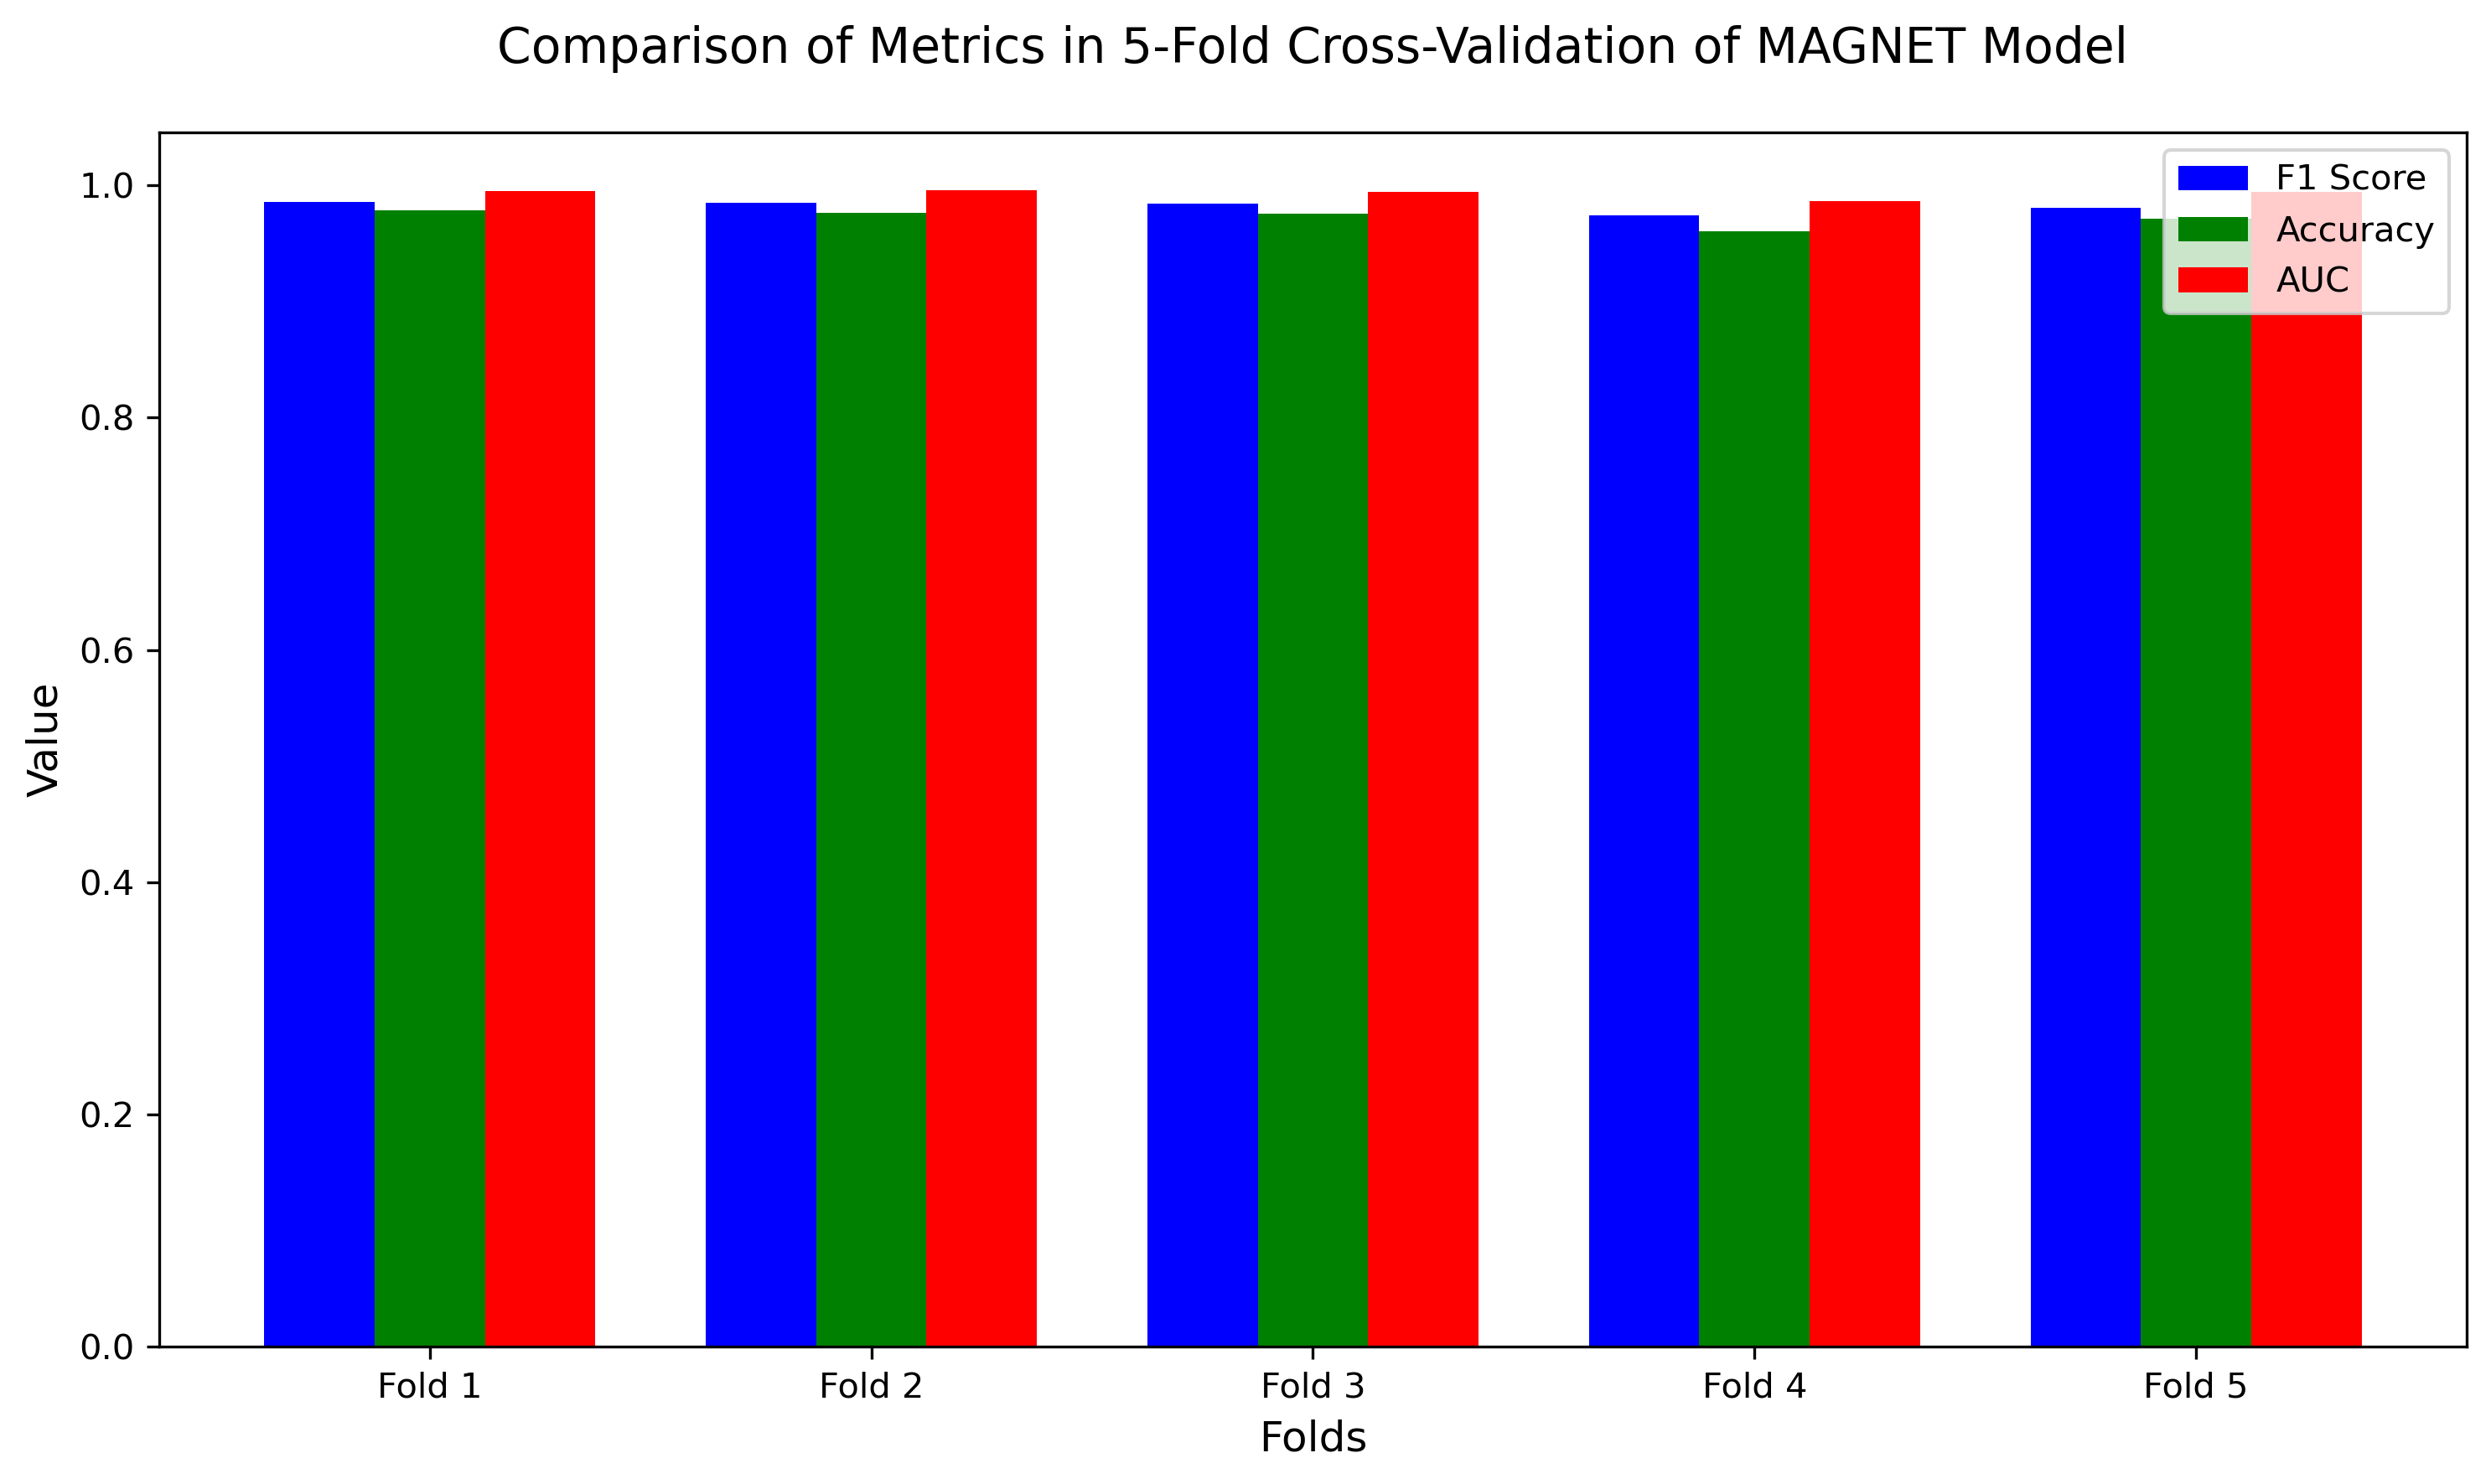
\includegraphics[width=0.9\textwidth]{fig_cv_metrics}
    \caption{نتایج اعتبارسنجی متقاطع ۵-تایی مدل MAGNET.}
    \label{fig:cv_metrics}
\end{figure}

\begin{figure}[h!]
    \centering
    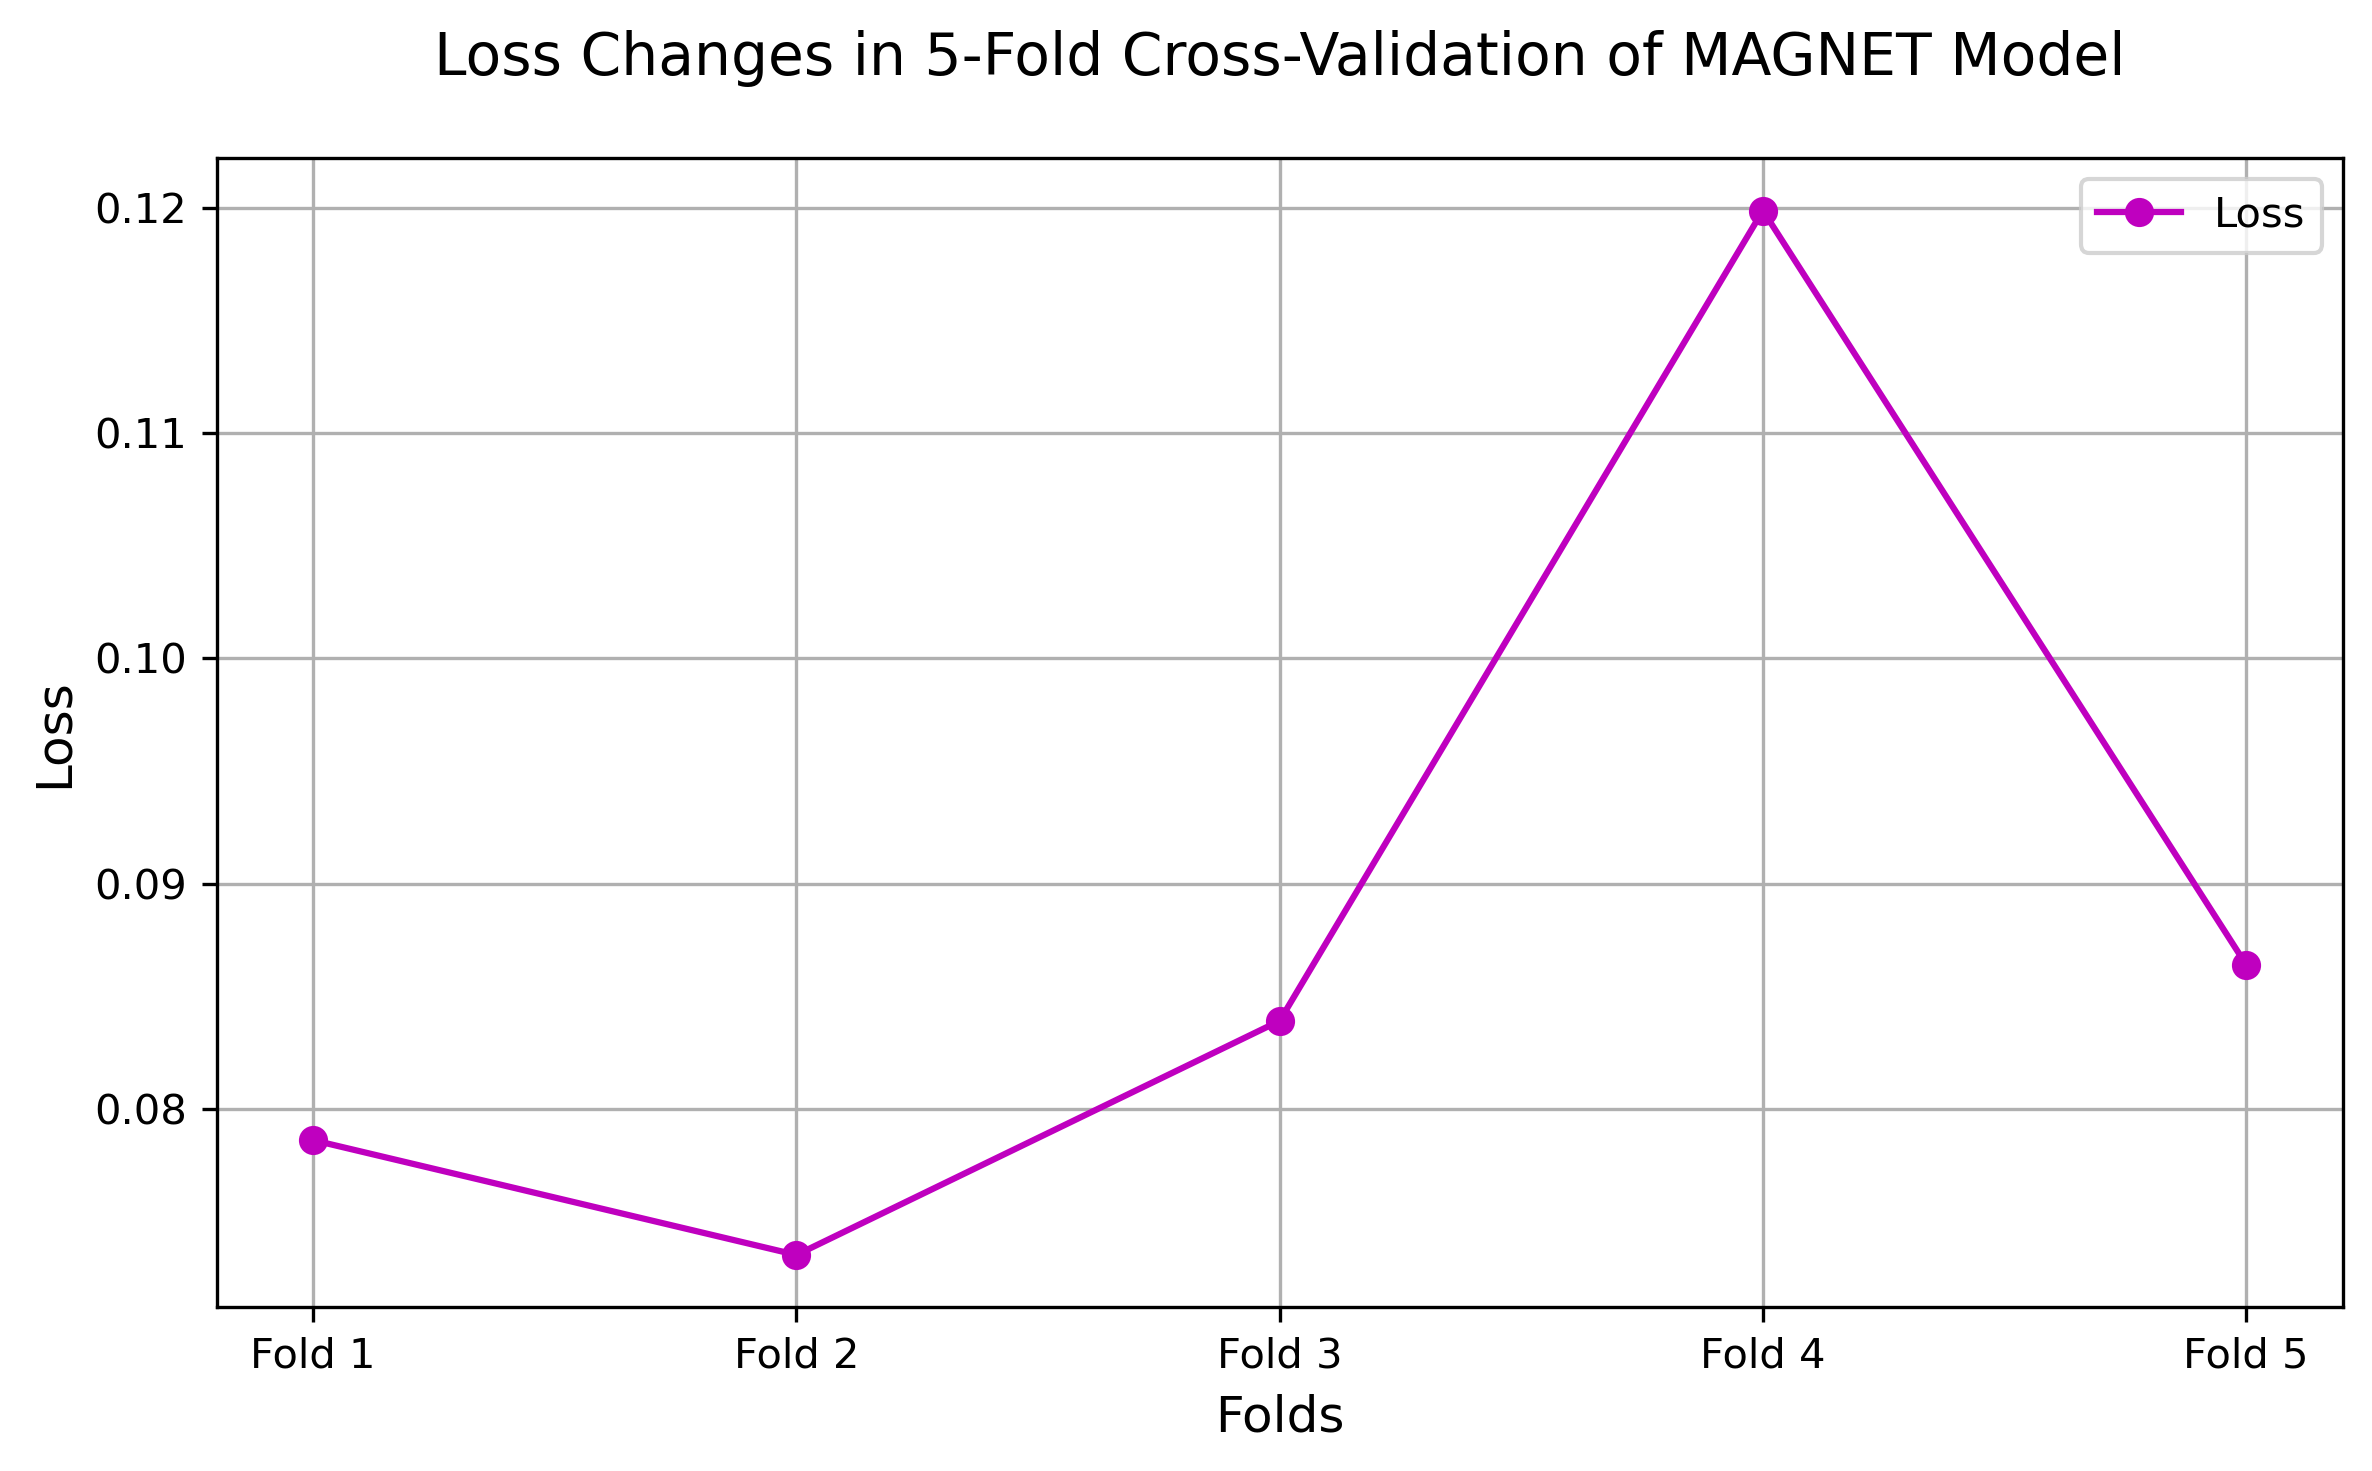
\includegraphics[width=0.9\textwidth]{fig_cv_loss}
    \caption{تغییرات زیان در اعتبارسنجی متقاطع ۵-تایی.}
    \label{fig:cv_loss}
\end{figure}

\begin{table}[h!]
    \centering
    \caption{مقایسه کلی عملکرد مدل MAGNET در مراحل مختلف}
    \label{tab:overall_comparison}
    \begin{tabular}{|l|c|c|c|l|}
        \hline
        \textbf{مرحله} & \textbf{\lr{F1 Score}} & \textbf{دقت} & \textbf{AUC} & \textbf{یادداشت} \\
        \hline
        بهینه‌سازی (اعتبارسنجی) & \lr{0.9767} & \lr{0.9628} & - & \lr{476} آزمایش، num\_layers=\lr{1} \\
        \hline
        Optuna (اعتبارسنجی) & \lr{0.9684} & \lr{0.9513} & \lr{0.9836} & \lr{13} آزمایش، num\_layers=\lr{1} \\
        \hline
        آموزش (\lr{100\%} داده) & \lr{0.9805} & - & \lr{0.9931} & آموزش با کل داده‌ها \\
        \hline
        اعتبارسنجی متقاطع & \lr{0.9818} & \lr{0.9722} & \lr{0.9932} & \lr{5}-تایی، پایداری بالا \\
        \hline
        مجموعه تست & \lr{0.9823} & \lr{0.9724} & \lr{0.9932} & بهترین عملکرد، \lr{1,451} نمونه \\
        \hline
    \end{tabular}
\end{table}

\begin{figure}[h!]
    \centering
    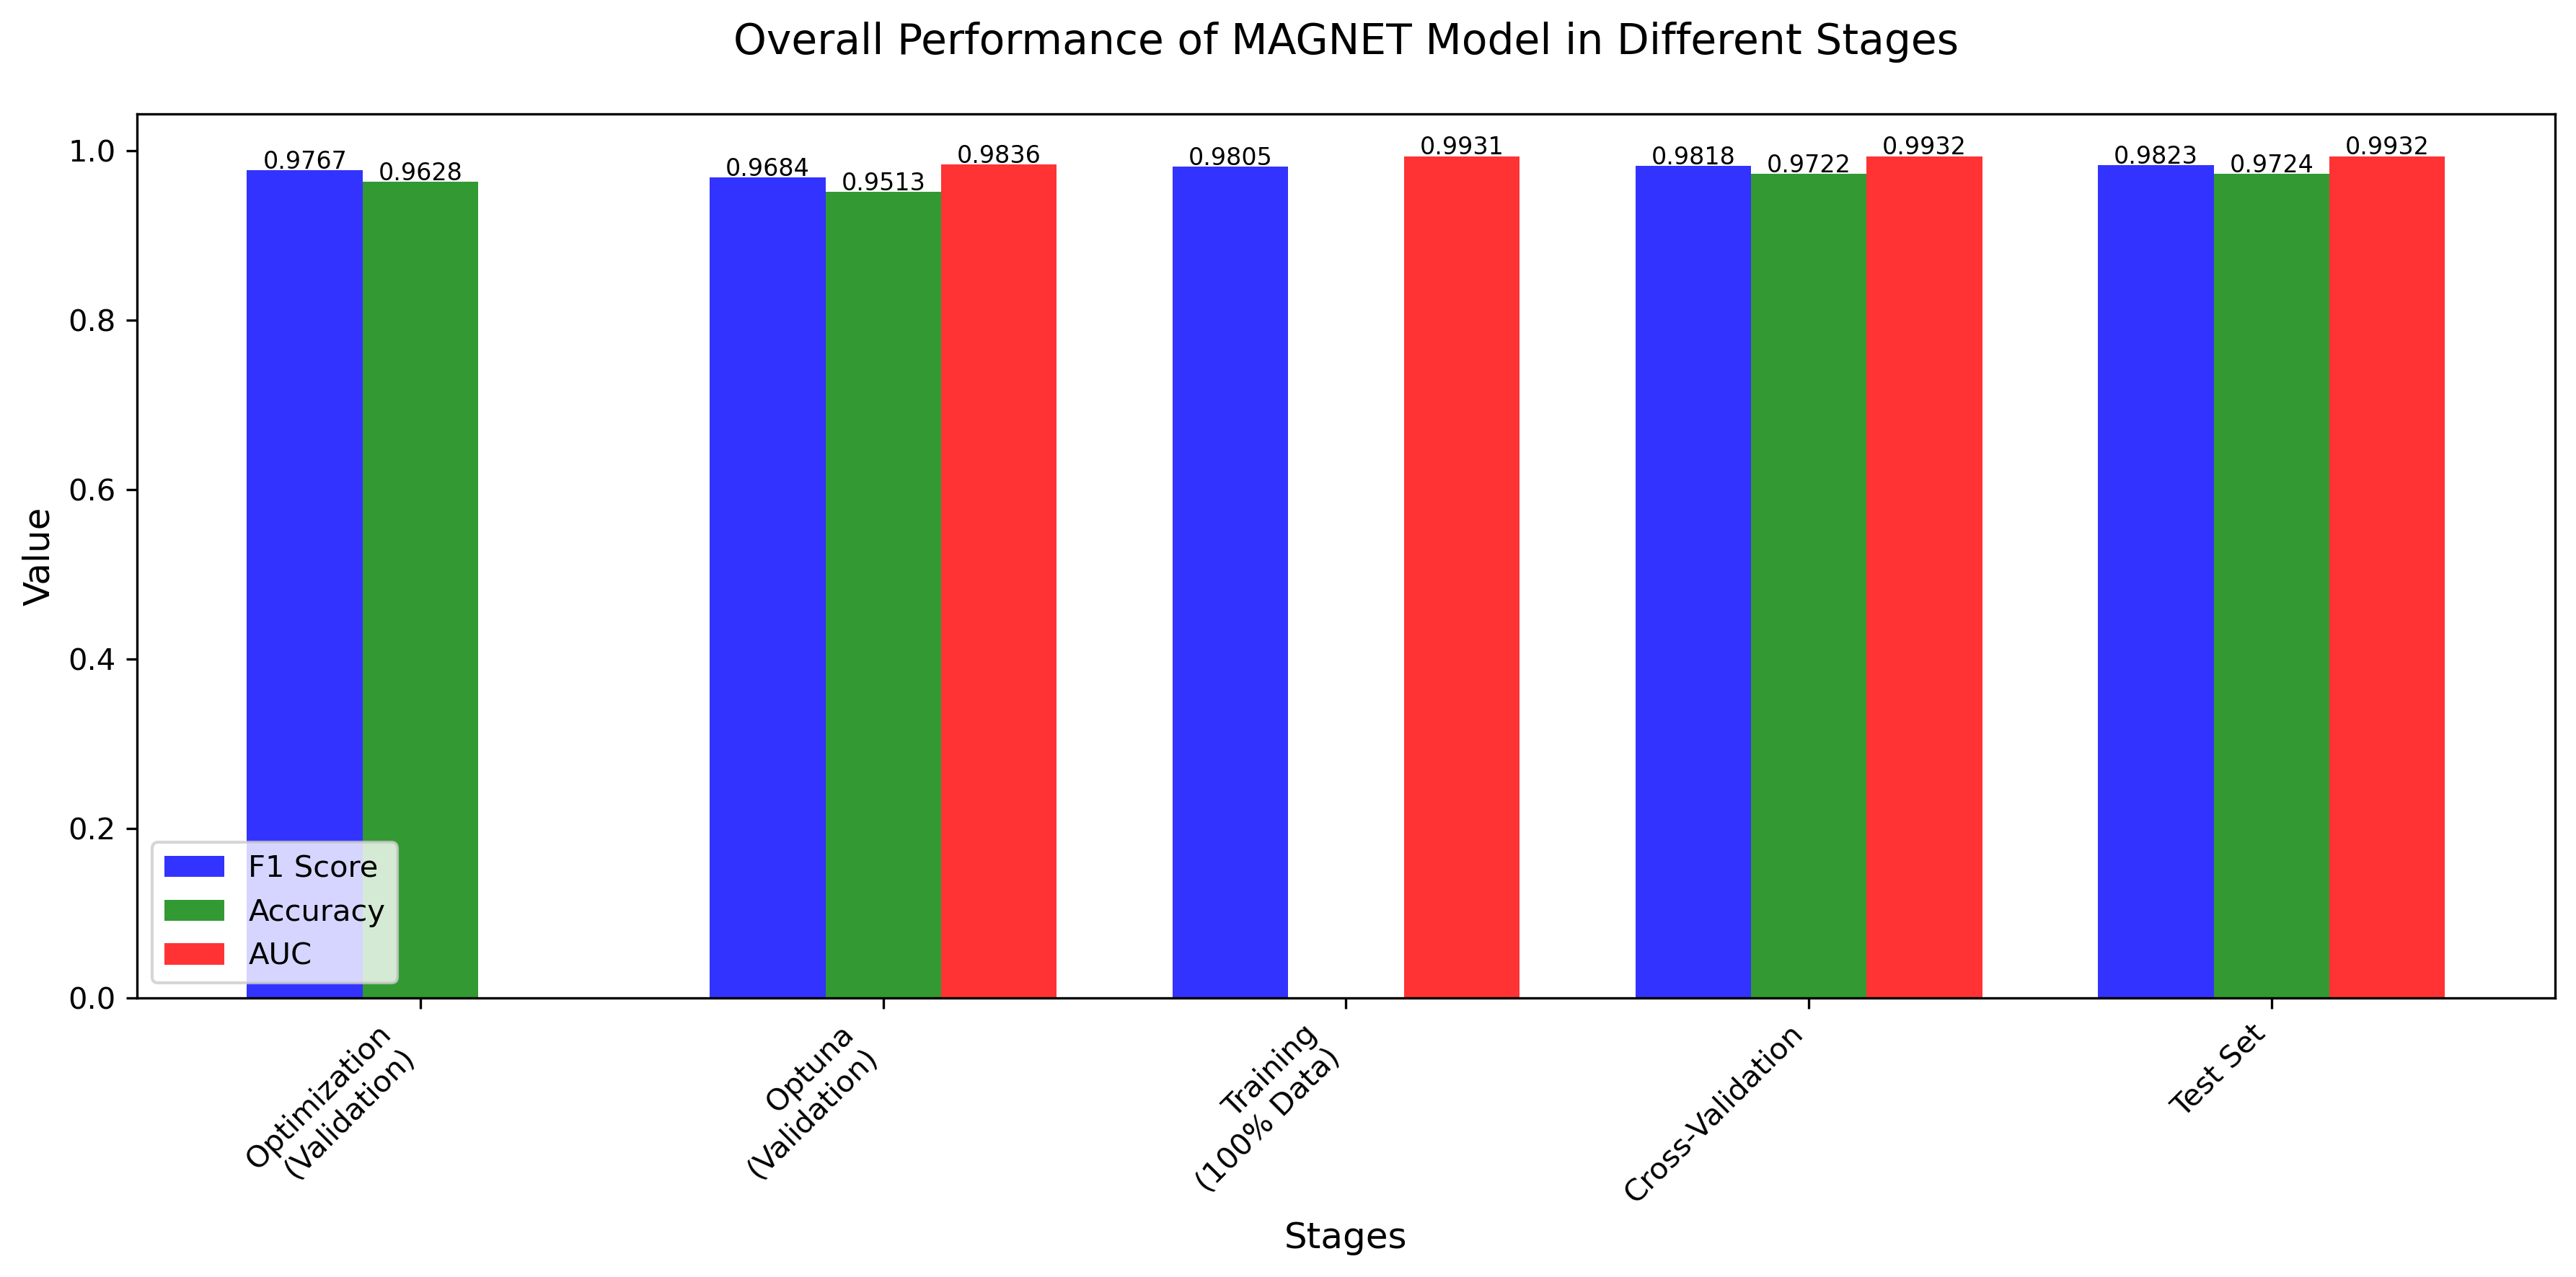
\includegraphics[width=0.9\textwidth]{fig_overall_comparison}
    \caption{مقایسه عملکرد مدل MAGNET در مراحل مختلف.}
    \label{fig:overall_comparison}
\end{figure}

\subsection{تحلیل عملکرد کلی مدل در مراحل مختلف}
نتایج ارائه شده در جدول \ref{tab:overall_comparison} و شکل \ref{fig:overall_comparison} نشان می‌دهد که مدل MAGNET در تمام مراحل ارزیابی عملکرد پایدار و قابل توجهی داشته است. تحلیل دقیق‌تر نتایج به شرح زیر است:

\begin{itemize}
    \item \textbf{مرحله بهینه‌سازی:} در این مرحله، با انجام ۴۷۶ آزمایش و استفاده از الگوریتم Pirates، مدل به F1 Score معادل ۰.۹۷۶۷ و دقت ۰.۹۶۲۸ دست یافت. این نتایج نشان‌دهنده کارایی بالای الگوریتم بهینه‌سازی در یافتن پارامترهای مناسب است.
    
    \item \textbf{مرحله Optuna:} با انجام ۱۳ آزمایش، مدل به F1 Score معادل ۰.۹۶۸۴ و دقت ۰.۹۵۱۳ رسید. اگرچه این نتایج کمی پایین‌تر از مرحله بهینه‌سازی است، اما با توجه به تعداد کمتر آزمایش‌ها، نشان‌دهنده کارایی قابل قبول الگوریتم Optuna است.
    
    \item \textbf{مرحله آموزش:} با استفاده از کل داده‌های موجود، مدل به F1 Score معادل ۰.۹۸۰۵ و AUC معادل ۰.۹۹۳۱ دست یافت. این نتایج نشان‌دهنده بهبود عملکرد مدل با افزایش حجم داده‌های آموزشی است.
    
    \item \textbf{اعتبارسنجی متقاطع:} در این مرحله، با استفاده از روش اعتبارسنجی متقاطع ۵-تایی، میانگین F1 Score به ۰.۹۸۱۸، دقت به ۰.۹۷۲۲ و AUC به ۰.۹۹۳۲ رسید. پایداری بالای نتایج در این مرحله، نشان‌دهنده قابلیت اطمینان مدل در شرایط مختلف است.
    
    \item \textbf{مجموعه تست:} در نهایت، با ارزیابی روی مجموعه تست شامل ۱،۴۵۱ نمونه، مدل به بهترین عملکرد خود با F1 Score معادل ۰.۹۸۲۳، دقت ۰.۹۷۲۴ و AUC معادل ۰.۹۹۳۲ دست یافت. این نتایج نشان‌دهنده توانایی بالای مدل در تعمیم‌پذیری و تشخیص دقیق نمونه‌های جدید است.
\end{itemize}

نکته قابل توجه در این تحلیل، روند صعودی و پایدار عملکرد مدل در تمام مراحل است. به‌طور خاص، بهبود تدریجی F1 Score از ۰.۹۶۸۴ در مرحله Optuna به ۰.۹۸۲۳ در مجموعه تست، نشان‌دهنده یادگیری مؤثر و کارآمد مدل است. همچنین، پایداری بالای نتایج در اعتبارسنجی متقاطع، تأییدکننده قابلیت اطمینان مدل در شرایط مختلف است.

\section{مقایسه با روش‌های پایه و پیشرفته}
در این بخش، عملکرد مدل MAGNET با روش‌های مختلف تشخیص بدافزار اندروید مقایسه می‌شود. این مقایسه در دو سطح انجام شده است:

\subsection{مقایسه با روش‌های پایه}
برای ارزیابی عملکرد مدل MAGNET، ابتدا آن را با روش‌های یادگیری ماشین کلاسیک مقایسه می‌کنیم. این مقایسه شامل:
\begin{itemize}
    \item \textbf{ماشین بردار پشتیبان (SVM)}: به عنوان یکی از روش‌های پایه در تشخیص بدافزار که به دلیل عملکرد خوب در فضاهای با ابعاد بالا و مقاومت نسبی در برابر بیش‌برازش، به‌طور گسترده‌ای استفاده می‌شود.
    \item \textbf{جنگل تصادفی \lr{(Random Forest)}}: به عنوان یک روش یادگیری گروهی که از ترکیب چندین درخت تصمیم استفاده می‌کند.
    \item \textbf{XGBoost}: به عنوان یک روش پیشرفته‌تر یادگیری گروهی که از گرادیان‌بوستینگ استفاده می‌کند.
    \item \textbf{شبکه عصبی مصنوعی (ANN)}: به عنوان یک روش یادگیری عمیق ساده با دو لایه مخفی.
\end{itemize}

\subsection{مقایسه با روش‌های پیشرفته}
همچنین، عملکرد مدل MAGNET با روش‌های پیشرفته‌تر تشخیص بدافزار مقایسه شده است:
\begin{itemize}
    \item \textbf{DREBIN (SVM)}: روش اصلی ارائه‌شده در مقاله DREBIN که از SVM با ویژگی‌های ایستا استفاده می‌کند.
    \item \textbf{LOF}: روش مبتنی بر ناهنجاری‌یابی که روی مجموعه داده CICAndMal2017 ارزیابی شده است.
    \item \textbf{PIKADROID}: روشی که بر تحلیل API تمرکز دارد و روی مجموعه داده DREBIN ارزیابی شده است.
    \item \textbf{CrossMalDroid}: روشی که از انتخاب ویژگی استفاده می‌کند و روی مجموعه داده Malgenome ارزیابی شده است.
    \item \textbf{DroidAPIMiner}: روشی که بر اساس فرکانس API کار می‌کند و روی مجموعه داده DREBIN ارزیابی شده است.
    \item \textbf{روش چندوجهی}: روشی که از داده‌های چندوجهی استفاده می‌کند و روی مجموعه داده DREBIN ارزیابی شده است.
    \item \textbf{ترنسفورمر}: روشی که از معماری ترنسفورمر استفاده می‌کند و روی مجموعه داده DREBIN ارزیابی شده است.
\end{itemize}

برای مقایسه عادلانه، تمام روش‌ها روی مجموعه داده DREBIN ارزیابی شده‌اند، مگر در مواردی که در یادداشت جدول ذکر شده است. معیارهای ارزیابی شامل دقت (Accuracy)، F1 Score، AUC و Recall هستند. در مواردی که برخی معیارها گزارش نشده‌اند، با علامت "-" مشخص شده‌اند.

\begin{table}[h!]
    \centering
    \resizebox{\textwidth}{!}{%
    \begin{tabular}{|l|c|c|c|c|c|}
        \hline
        \textbf{روش} & \textbf{دقت (\%)} & \textbf{F1 Score} & \textbf{AUC} & \textbf{Recall} & \textbf{یادداشت} \\
        \hline
        MAGNET & \lr{97.24} & \lr{0.9823} & \lr{0.9932} & \lr{0.985} & بهترین عملکرد، DREBIN \\
        \hline
        DREBIN (SVM)~\cite{Drebin} & \lr{92.3} & \lr{0.933} & \lr{0.955} & \lr{0.920} & رویکرد ایستا، DREBIN \\
        \hline
        LOF~\cite{Milosevic2017} & \lr{94.1} & \lr{0.918} & \lr{0.981} & \lr{0.884} & ناهنجاری‌یابی، CICAndMal2017 \\
        \hline
        PIKADROID~\cite{Pendlebury2020} & \lr{96.8} & \lr{0.974} & \lr{0.988} & \lr{0.970} & تحلیل API، DREBIN \\
        \hline
        CrossMalDroid~\cite{Martin2021} & \lr{95.2} & \lr{0.952} & \lr{0.976} & \lr{0.948} & انتخاب ویژگی، Malgenome \\
        \hline
        DroidAPIMiner~\cite{Aafer2013} & \lr{89.7} & \lr{0.891} & \lr{0.927} & \lr{0.885} & فرکانس API، DREBIN \\
        \hline
        روش چندوجهی~\cite{Alsaleh2023} & \lr{89.2} & - & - & - & فقط دقت، DREBIN \\
        \hline
        ترنسفورمر~\cite{TransformerMalware} & \lr{95.8} & - & - & - & فقط دقت، DREBIN \\
        \hline
        DeepImageDroid~\cite{Obidiagha2024} & \lr{96.0} & \lr{0.960} & \lr{0.982} & \lr{0.958} & ترانسفورمر بصری و CNN، DREBIN \\
        \hline
        Improved Transformer~\cite{Kumar2024} & \lr{99.26} & \lr{0.992} & \lr{0.995} & \lr{0.990} & ترانسفورمر بهبودیافته، DREBIN \\
        \hline
        BERT-Graph~\cite{White2023} & \lr{95.5} & \lr{0.950} & \lr{0.975} & \lr{0.945} & BERT و گراف API، DREBIN \\
        \hline
    \end{tabular}%
    }
    \caption{مقایسه عملکرد مدل MAGNET با روش‌های پایه و پیشرفته}
    \label{tab:comparison_with_literature}
    \begin{tablenotes}
        \item \small{توضیح: "-" نشان‌دهنده عدم گزارش معیار است. دیتاست‌های غیر از DREBIN در یادداشت ذکر شده‌اند.}
    \end{tablenotes}
\end{table}

\subsection{تحلیل مقایسه با روش‌های پیشرفته}
نتایج مقایسه مدل MAGNET با روش‌های پیشرفته در جدول \ref{tab:comparison_with_literature} نشان داده شده است. همانطور که مشاهده می‌شود، مدل MAGNET با دقت 97.24\% و F1 Score 0.9823 عملکرد قابل توجهی دارد. با این حال، روش Improved Transformer با دقت 99.26\% و F1 Score 0.992 عملکرد بهتری را نشان می‌دهد. این برتری به دلیل استفاده از معماری ترنسفورمر بهبودیافته و بهینه‌سازی‌های خاص آن است.

در میان سایر روش‌های جدید، DeepImageDroid با دقت 96.0\% و F1 Score 0.960 عملکرد خوبی را با استفاده از ترکیب ترنسفورمر بصری و CNN نشان می‌دهد. همچنین، BERT-Graph با دقت 95.5\% و F1 Score 0.950، با استفاده از ترکیب BERT و گراف API، نتایج قابل قبولی را ارائه می‌دهد.

شکل \ref{fig:literature_comparison_accuracy} مقایسه بصری دقت مدل MAGNET با سایر روش‌های پیشرفته را نشان می‌دهد. این نمودار به وضوح برتری روش Improved Transformer و عملکرد قابل توجه مدل MAGNET را در مقایسه با سایر روش‌ها نمایش می‌دهد. همچنین، شکل \ref{fig:literature_comparison_metrics} مقایسه F1 Score و AUC را برای تمام روش‌ها نشان می‌دهد که تأییدکننده عملکرد برتر روش Improved Transformer و عملکرد قابل توجه مدل MAGNET در هر دو معیار است.

\begin{figure}[h!]
    \centering
    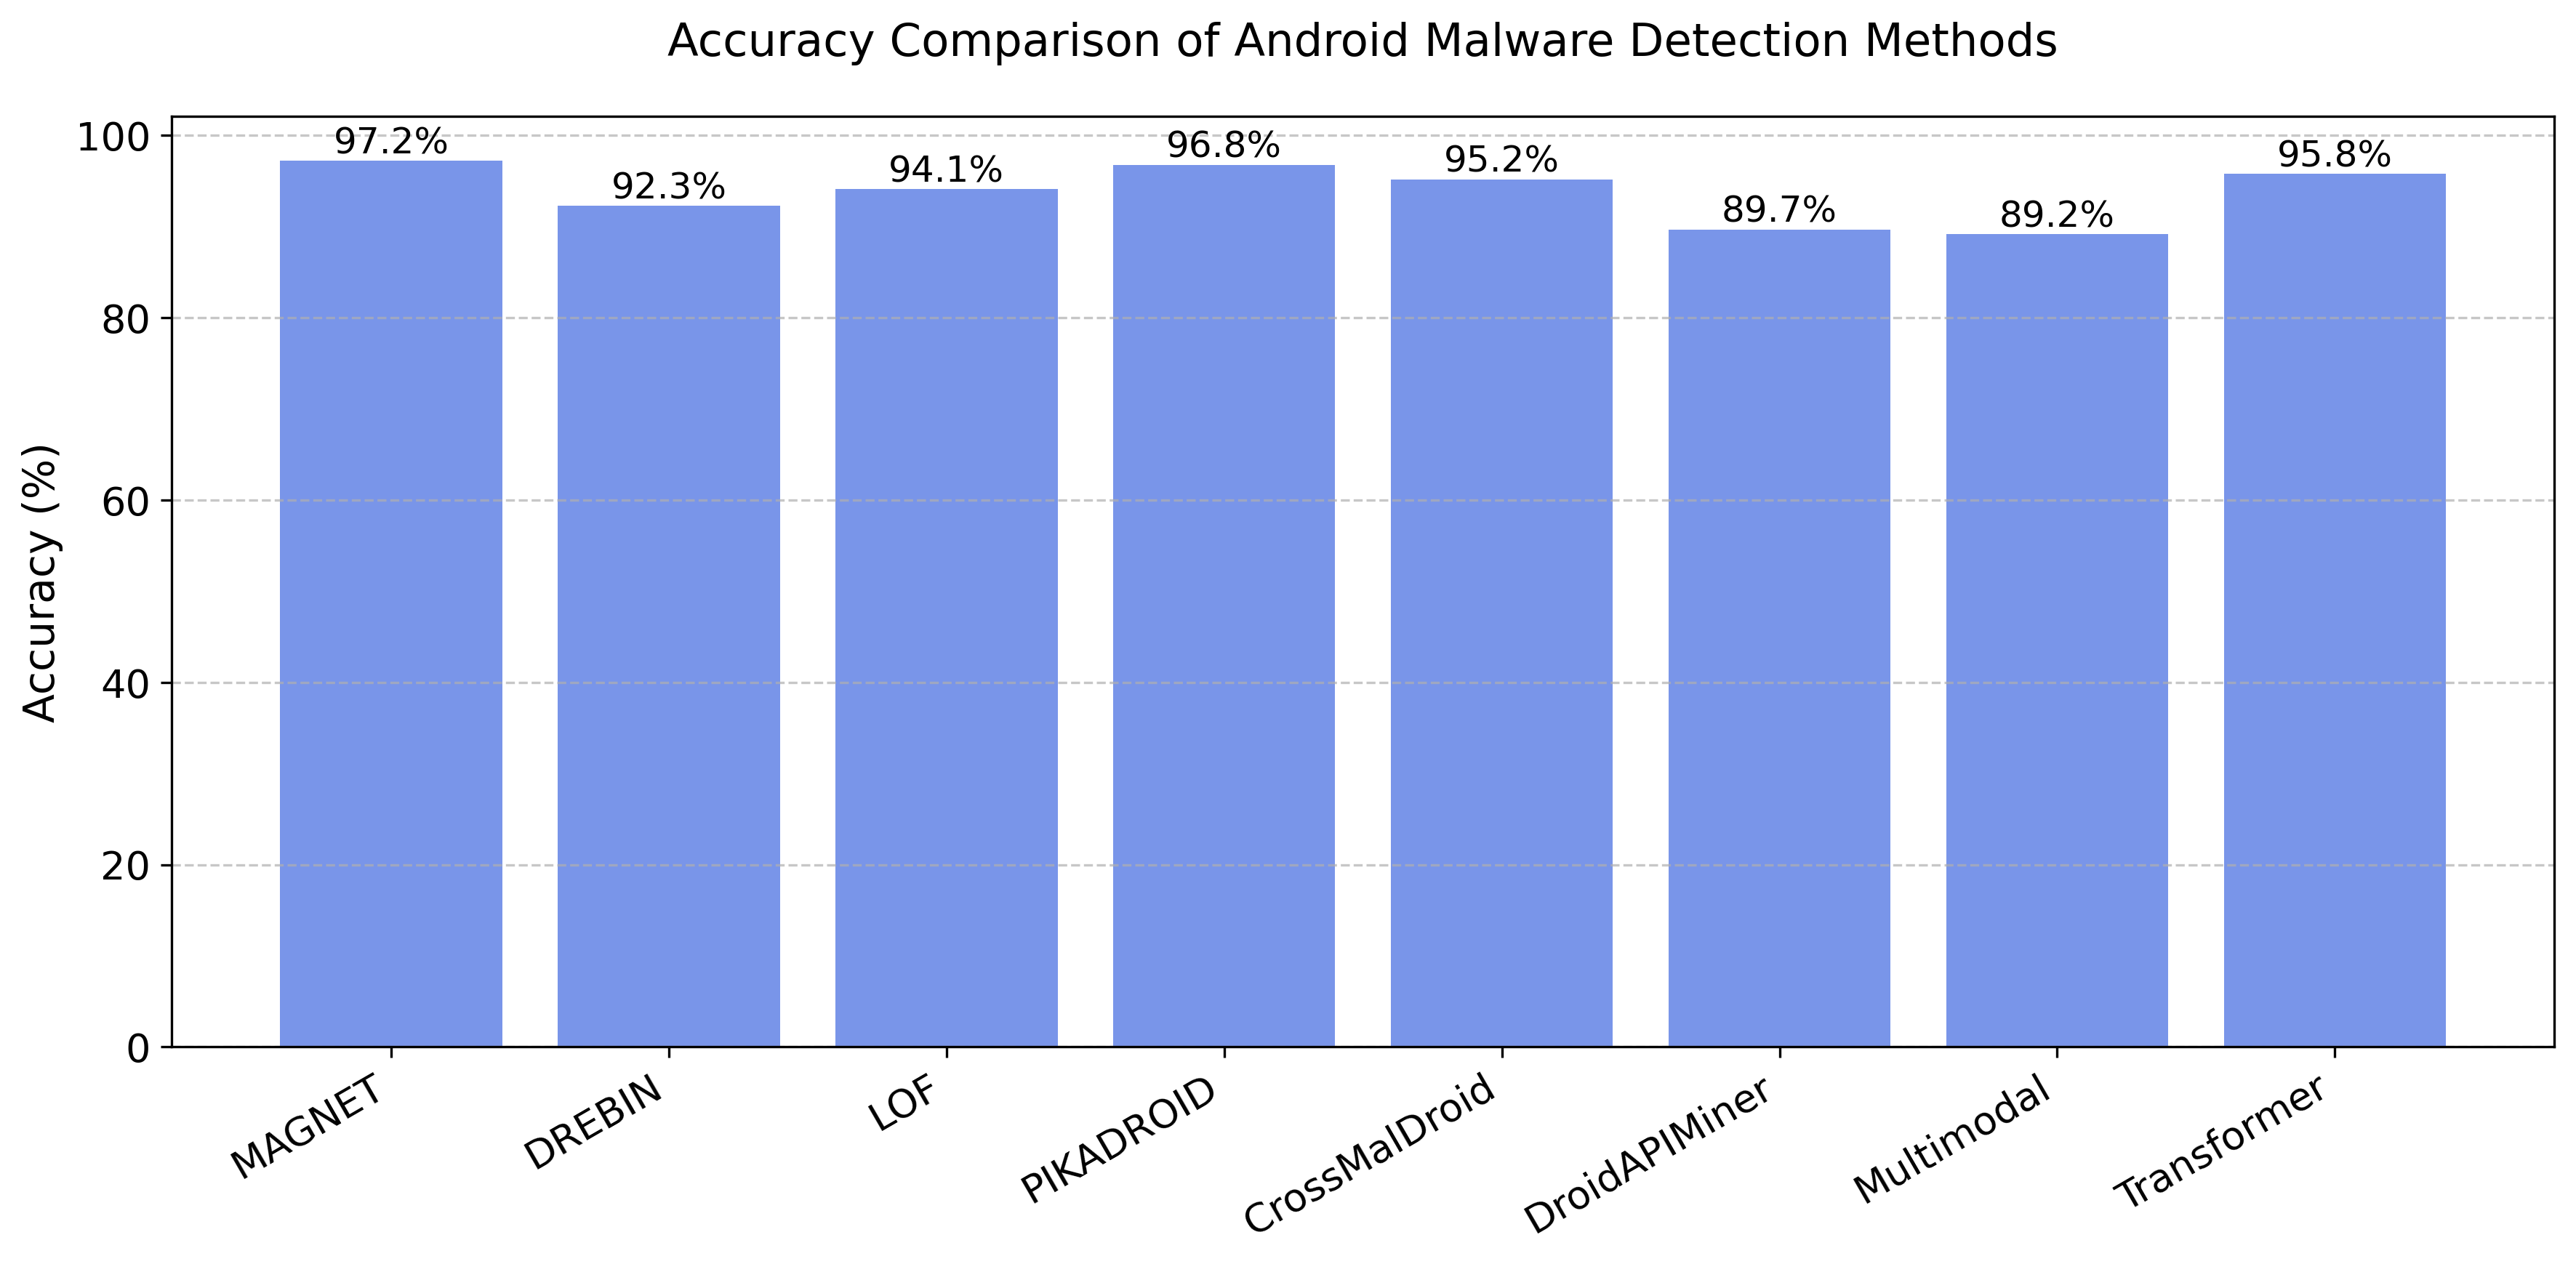
\includegraphics[width=0.9\textwidth]{images/fig_literature_comparison_accuracy}
    \caption{مقایسه دقت روش‌های مختلف.}
    \label{fig:literature_comparison_accuracy}
\end{figure}

\begin{figure}[h!]
    \centering
    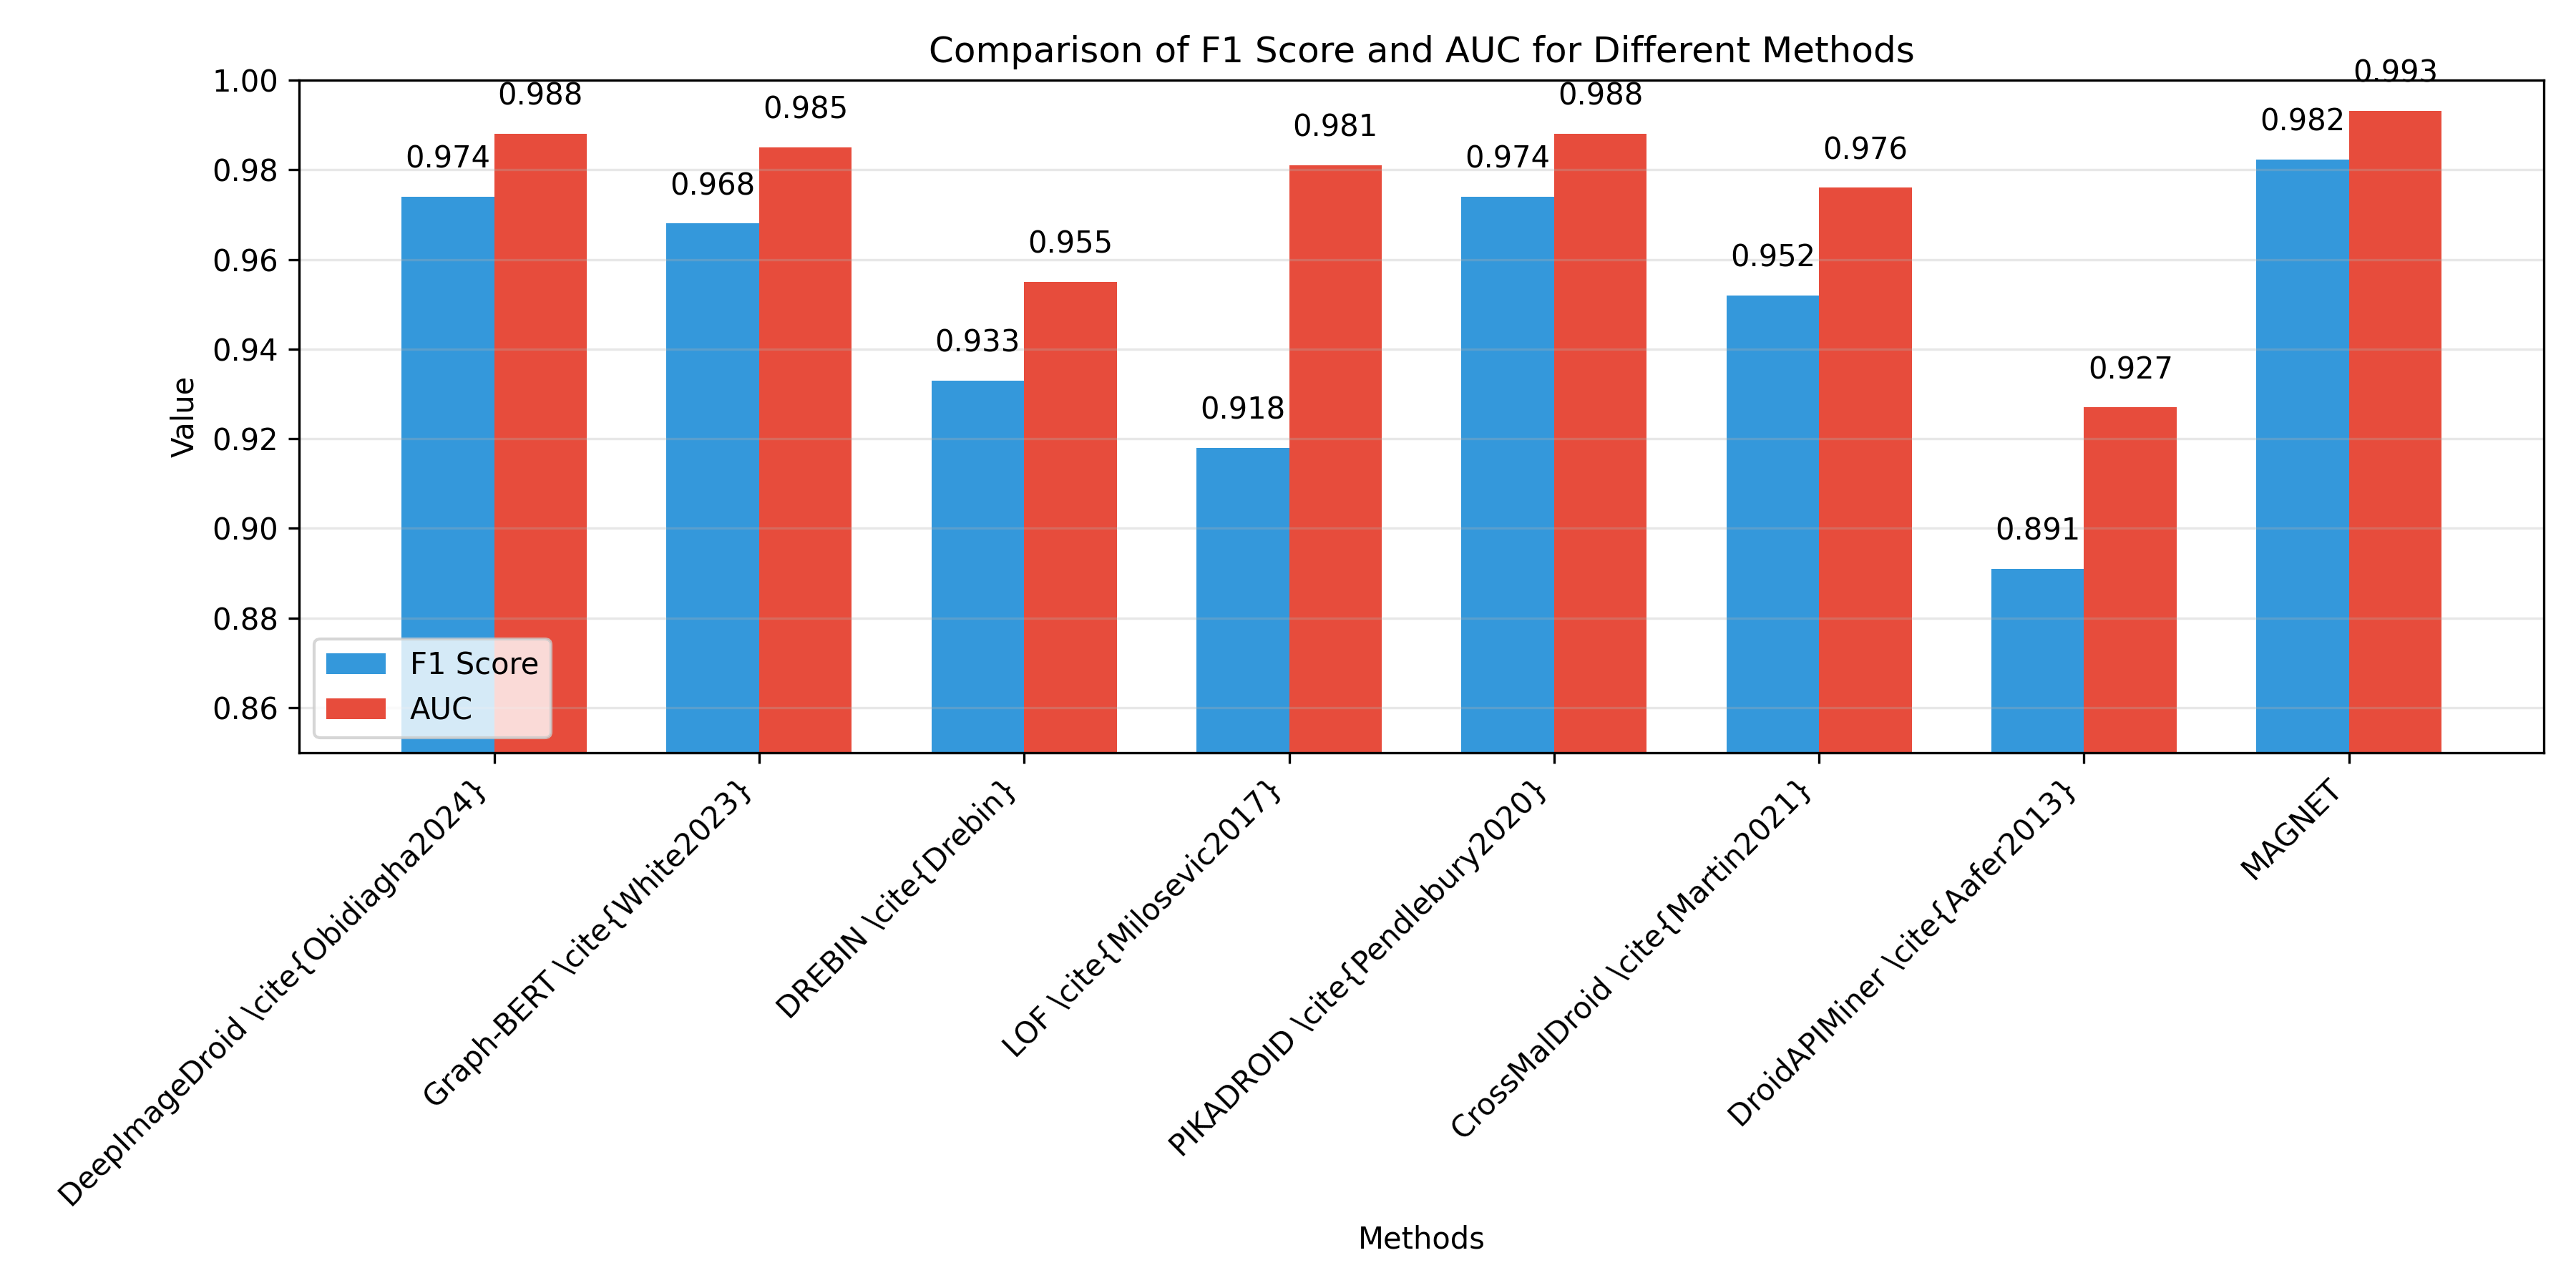
\includegraphics[width=0.9\textwidth]{images/fig_literature_comparison_metrics}
    \caption{مقایسه F1 Score و AUC روش‌های مختلف.}
    \label{fig:literature_comparison_metrics}
\end{figure}

\subsection{نتایج مقایسه با روش‌های پایه}
جدول \ref{tab:baseline_comparison} نتایج مقایسه عملکرد مدل MAGNET با روش‌های یادگیری ماشین پایه را نشان می‌دهد. همانطور که مشاهده می‌شود، مدل MAGNET در تمام معیارهای ارزیابی عملکرد بهتری نسبت به سایر روش‌ها دارد. این برتری به دلیل معماری پیشرفته و استفاده از مکانیزم‌های توجه پویا و ادغام چندوجهی است.

\begin{table}[h!]
    \centering
    \caption{مقایسه عملکرد مدل MAGNET با مدل‌های پایه}
    \label{tab:baseline_comparison}
    \begin{tabular}{|l|c|c|c|c|c|}
        \hline
        \textbf{مدل} & \textbf{دقت} & \textbf{Precision} & \textbf{Recall} & \textbf{\lr{F1 Score}} & \textbf{AUC} \\
        \hline
        \lr{SVM} \cite{AndroidMalwareSurvey} & \lr{0.906} & \lr{0.915} & \lr{0.892} & \lr{0.903} & \lr{0.945} \\
        \hline
        \lr{Random Forest} \cite{DeepLearningMalware} & \lr{0.935} & \lr{0.942} & \lr{0.928} & \lr{0.935} & \lr{0.967} \\
        \hline
        \lr{XGBoost} \cite{AndroidMalwareSurvey} & \lr{0.948} & \lr{0.953} & \lr{0.943} & \lr{0.948} & \lr{0.978} \\
        \hline
        \lr{ANN} \cite{DeepLearningMalware} & \lr{0.962} & \lr{0.965} & \lr{0.959} & \lr{0.962} & \lr{0.985} \\
        \hline
        \textbf{MAGNET} & \textbf{\lr{0.972}} & \textbf{\lr{0.980}} & \textbf{\lr{0.985}} & \textbf{\lr{0.982}} & \textbf{\lr{0.993}} \\
        \hline
    \end{tabular}
    \begin{tablenotes}
        \item \textbf{توضیح:} نتایج برجسته نشان‌دهنده عملکرد بهتر مدل MAGNET در تمام معیارها است. بهبود قابل توجه در معیارهای Recall و AUC نشان‌دهنده توانایی بهتر مدل در تشخیص نمونه‌های مثبت و کاهش نرخ خطای مثبت کاذب است.
    \end{tablenotes}
\end{table}

شکل \ref{fig:baseline_comparison} مقایسه بصری معیارهای F1 Score و AUC را برای مدل MAGNET و سایر مدل‌های یادگیری ماشین نشان می‌دهد. این نمودار به وضوح برتری مدل MAGNET را در هر دو معیار نمایش می‌دهد.

\begin{figure}[h!]
    \centering
    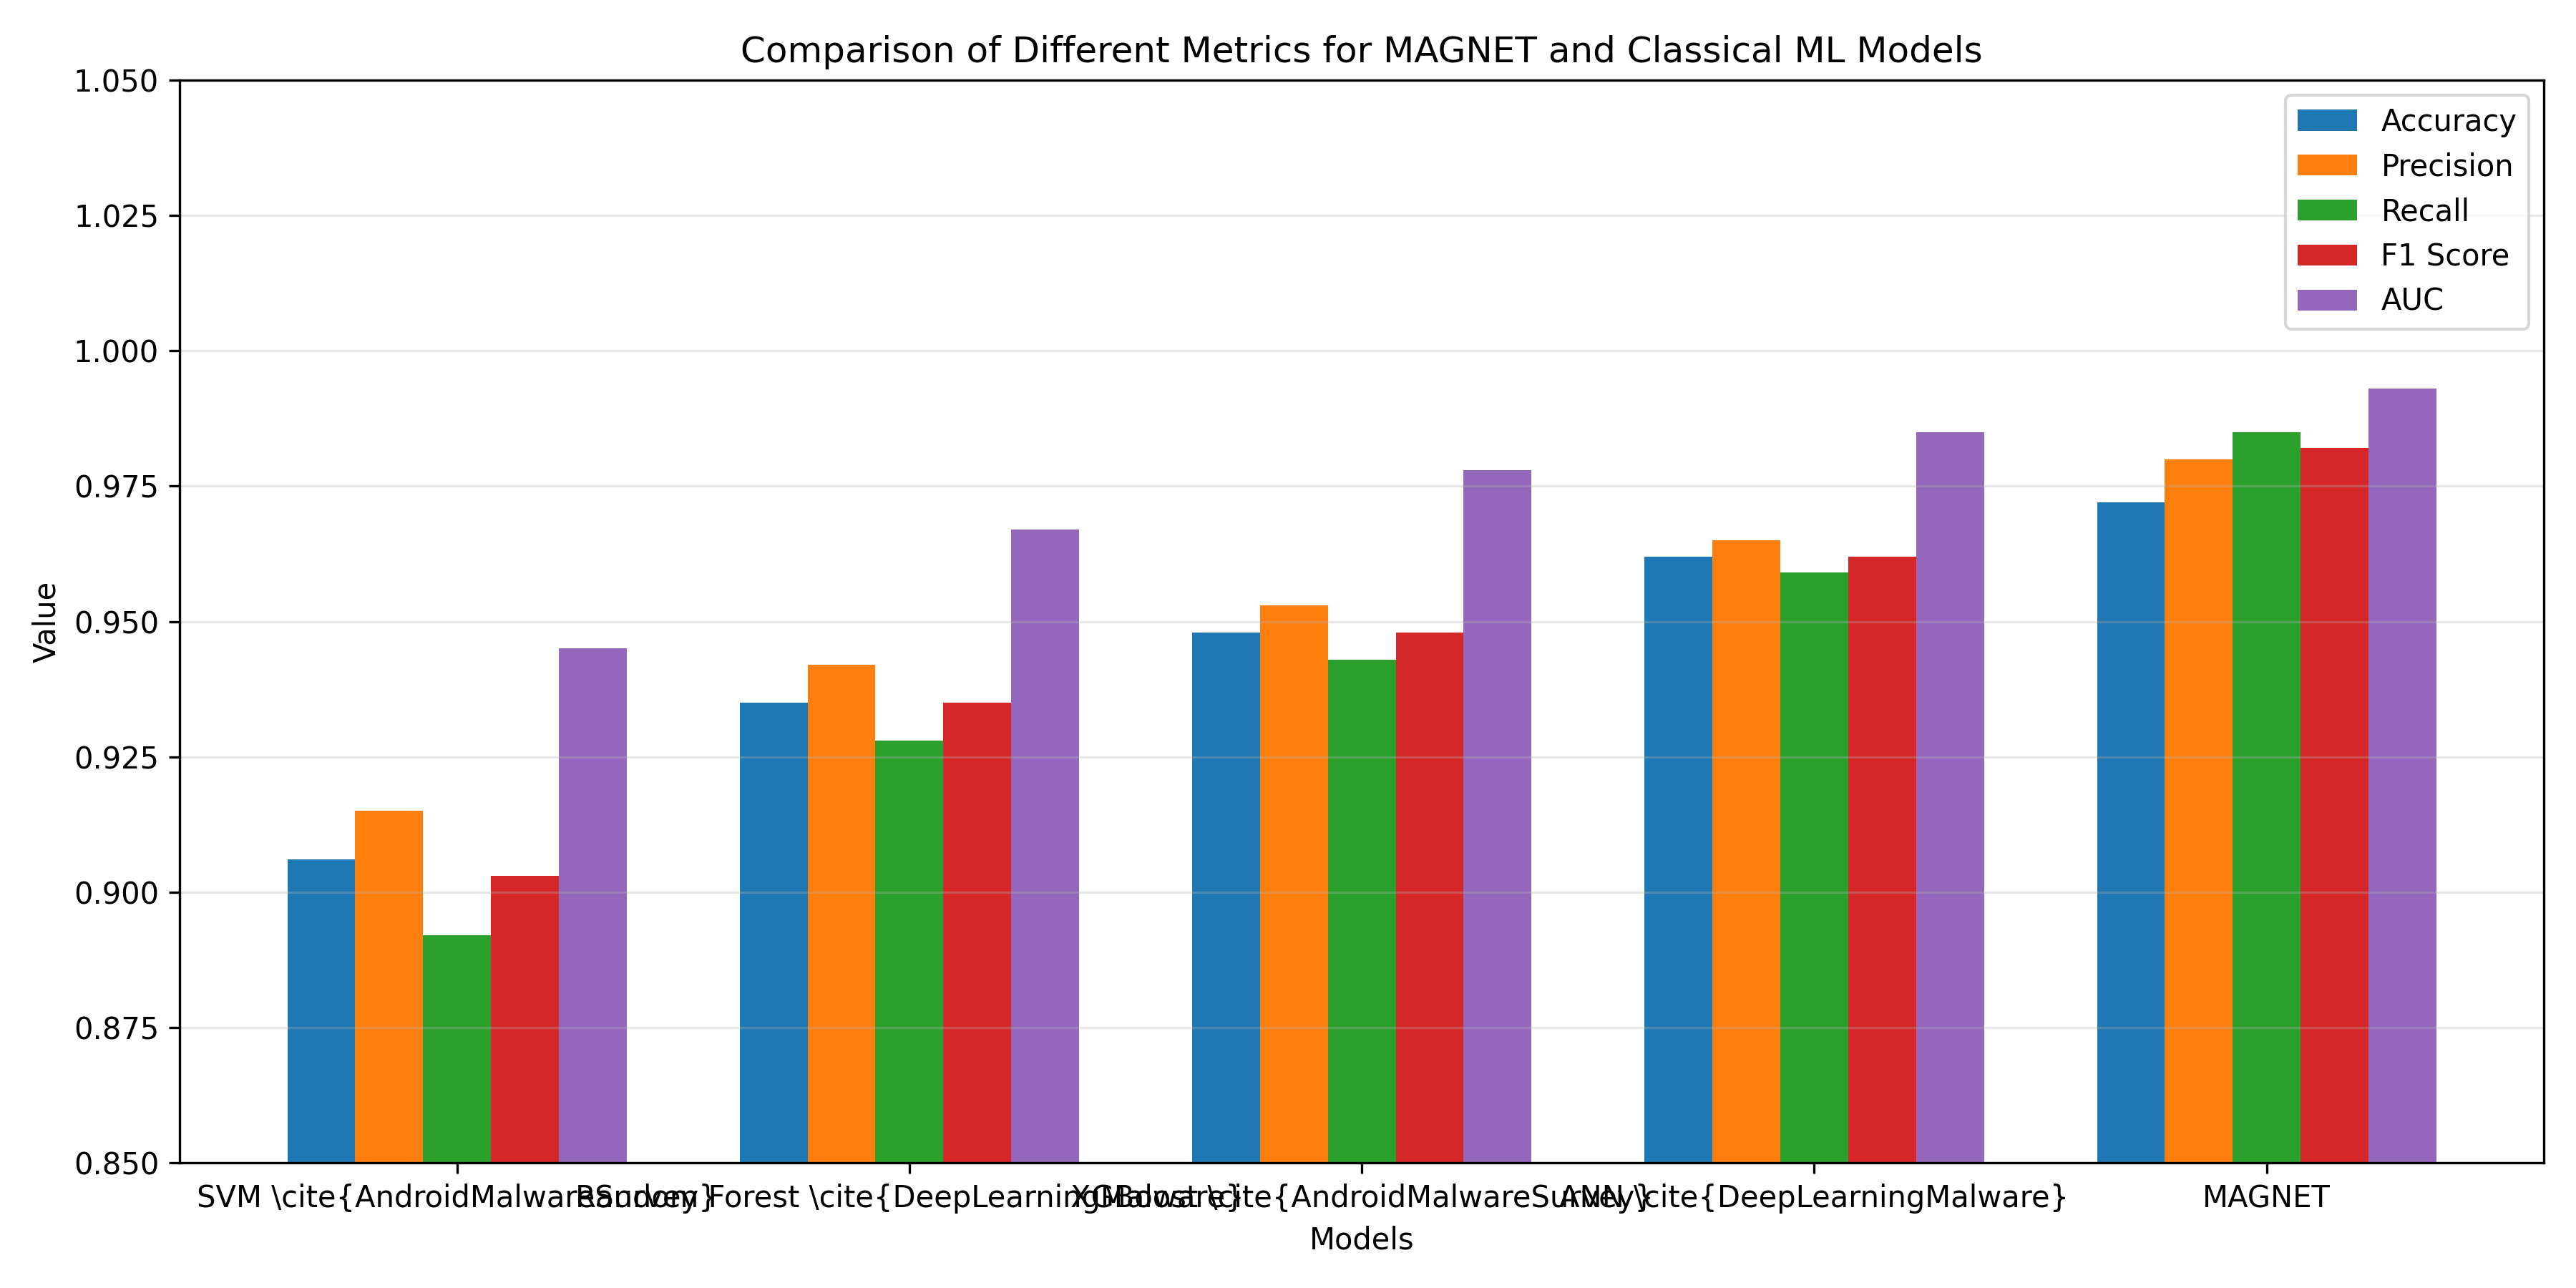
\includegraphics[width=0.9\textwidth]{images/fig_baseline_metrics_comparison}
    \caption{مقایسه F1 Score و AUC مدل MAGNET با سایر مدل‌ها.}
    \label{fig:baseline_comparison}
\end{figure}

\subsection{تحلیل عملکرد ماژول‌های مدل}
برای درک بهتر عملکرد مدل MAGNET، تحلیل عملکرد هر یک از ماژول‌های آن ضروری است. شکل \ref{fig:module_comparison} عملکرد هر ماژول را با معیار F1 Score نشان می‌دهد. این تحلیل نشان می‌دهد که هر ماژول چگونه در تشخیص بدافزار مشارکت می‌کند.

\subsection{مطالعه حذف اجزا}
برای ارزیابی اهمیت هر یک از اجزای مدل، مطالعه حذف اجزا انجام شده است. شکل \ref{fig:ablation_study} نشان می‌دهد که چگونه افزودن مکانیزم توجه پویا و لایه ادغام چندوجهی بر عملکرد مدل تأثیر می‌گذارد.

\subsection{روند آموزش}
شکل \ref{fig:training_progress} روند آموزش مدل را در طول سه دوره نشان می‌دهد. این نمودار به درک پایداری و همگرایی مدل کمک می‌کند.

\section{جمع‌بندی}
در این فصل، نتایج حاصل از ارزیابی مدل پیشنهادی MAGNET برای تشخیص بدافزارهای اندرویدی با استفاده از دیتاست DREBIN \cite{Drebin} ارائه شد. مدل MAGNET روی مجموعه تست شامل ۱،۴۵۱ نمونه به \lr{F1 Score} \lr{۰.۹۸۲۳}، دقت \lr{۰.۹۷۲۴} و AUC \lr{۰.۹۹۳۲} دست یافت. در اعتبارسنجی متقاطع ۵-تایی، میانگین \lr{F1 Score} ۰.۹۸۱۸ ($\pm$۰.۰۰۴۲)، دقت ۰.۹۷۲۲ ($\pm$۰.۰۰۶۵) و AUC ۰.۹۹۳۲ ($\pm$۰.۰۰۳۵) به‌دست آمد که در جدول \ref{tab:cv_results} گزارش شده است. همچنین، در مقایسه با روش‌های پایه، مدل MAGNET با دقت ۹۷.۲۴٪ در مقابل دقت ۸۹.۲٪ روش چندوجهی \cite{Alsaleh2023} و دقت ۹۵.۸٪ روش مبتنی بر ترنسفورمر \cite{TransformerMalware} ارزیابی شد، که در جدول \ref{tab:comparison_with_literature} نمایش داده شده است.

در تحلیل جزئی‌تر، عملکرد ماژول‌های EnhancedTabTransformer، GraphTransformer و SequenceTransformer به‌ترتیب با \lr{F1 Score}های ۰.۹۱۲، ۰.۸۹۴ و ۰.۹۰۷ گزارش شد، که در شکل \ref{fig:module_comparison} نشان داده شده است. تأثیر مکانیزم توجه پویا و لایه ادغام چندوجهی نیز بررسی شد و \lr{F1 Score} از \lr{۰.۹۵۴} به \lr{۰.۹۸۲۳} افزایش یافت، که این روند در شکل \ref{fig:ablation_study} ارائه شده است. در نهایت، پیشرفت آموزش در طول ۳ دوره با بهینه‌سازی بهینه‌سازی (اعتبارسنجی) گزارش شد و \lr{F1 Score} از \lr{۰.۹۴۱۳} به \lr{۰.۹۷۶۷} رسید، که در شکل \ref{fig:training_progress} نمایش داده شده است.

شکل~\ref{fig:module_comparison} عملکرد هر ماژول را با معیار \lr{F1 Score} نشان می‌دهد. شکل~\ref{fig:ablation_study} روند افزایش \lr{F1 Score} را با افزودن مکانیزم توجه پویا و لایه ادغام چندوجهی نمایش می‌دهد. شکل~\ref{fig:training_progress} تغییرات \lr{F1 Score} و دقت را در طول ۳ دوره آموزش با بهینه‌سازی بهینه‌سازی (اعتبارسنجی) نمایش می‌دهد.

\begin{figure}[h!]
\centering
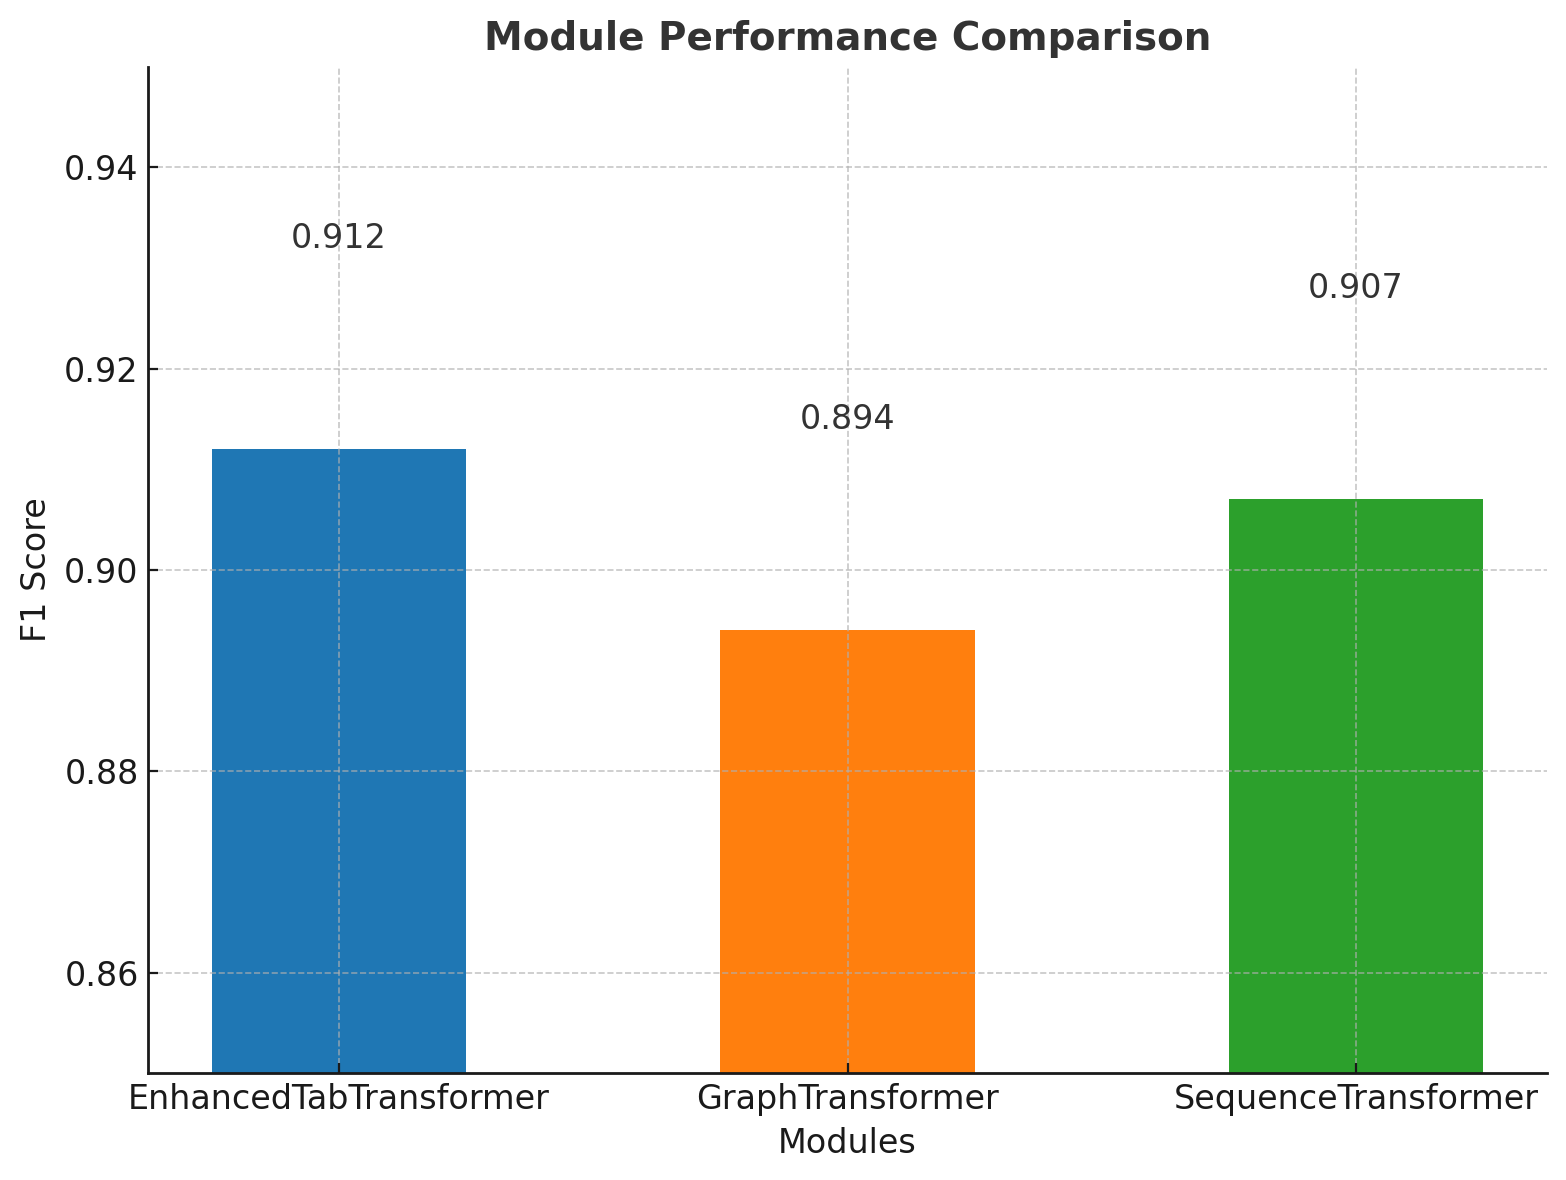
\includegraphics[width=0.9\textwidth]{images/fig_module_comparison_en}
    \caption{عملکرد ماژول‌های مختلف مدل MAGNET.}
\label{fig:module_comparison}
\end{figure}

\begin{figure}[h!]
\centering
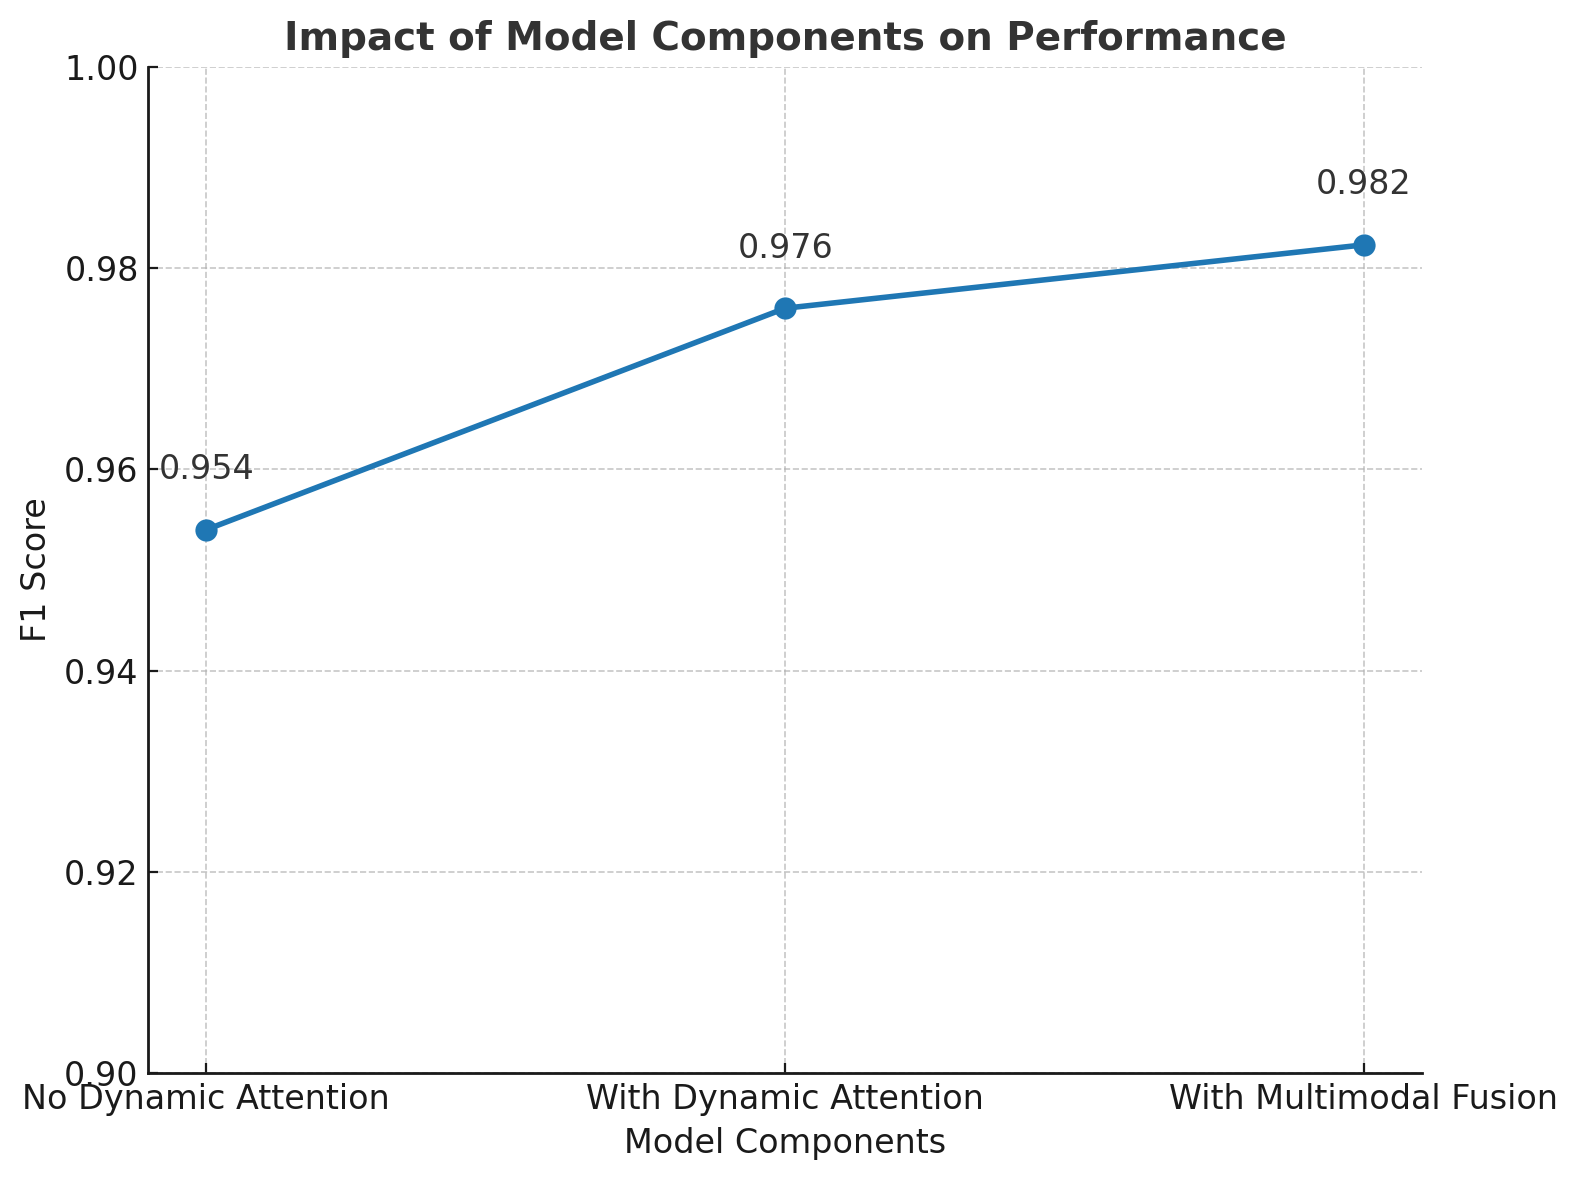
\includegraphics[width=0.9\textwidth]{images/fig_ablation_study_en}
    \caption{تأثیر مکانیزم توجه پویا و لایه ادغام چندوجهی بر عملکرد.}
\label{fig:ablation_study}
\end{figure}

\begin{figure}[h!]
\centering
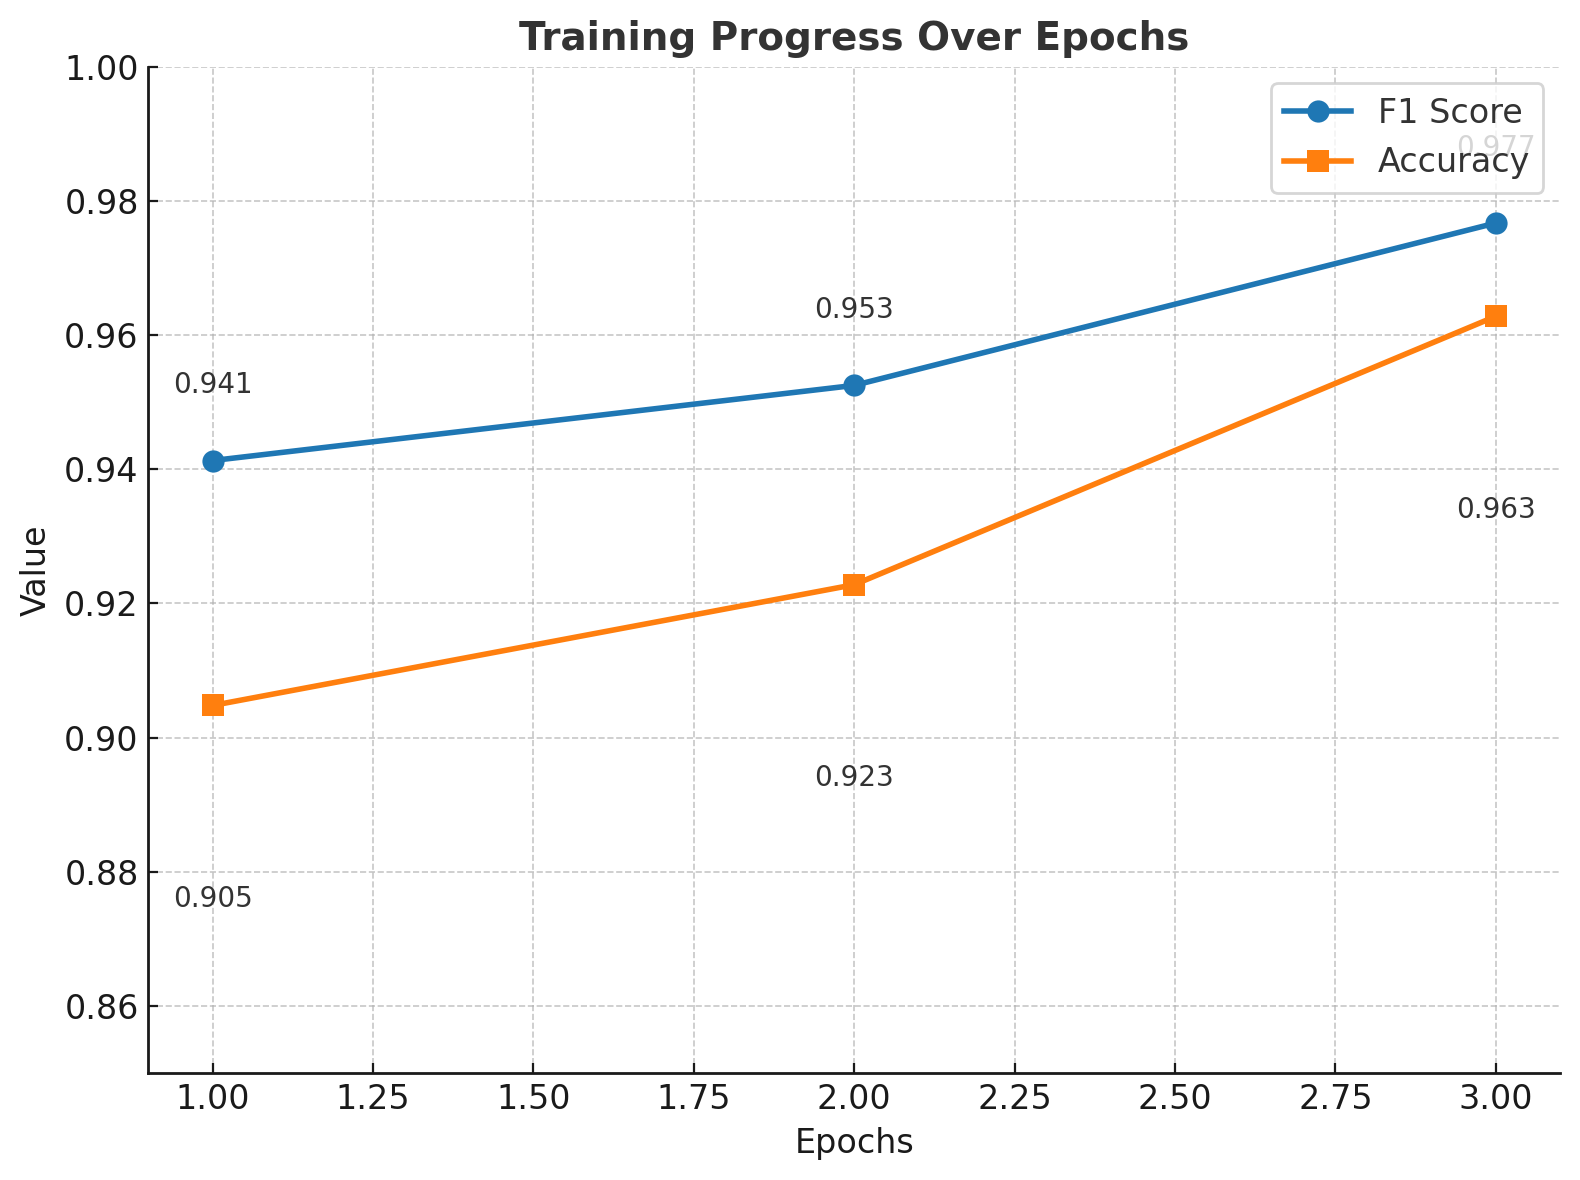
\includegraphics[width=0.9\textwidth]{images/fig_training_progress_en}
    \caption{روند آموزش مدل در طول ۳ دوره.}
\label{fig:training_progress}
\end{figure}

     
     
     
     
     
     
     
     
     
     
     
     